% !TeX spellcheck = en_US
\documentclass[RAIstudentthesis%      style
              ,optCharter%            font
              ,optBlackHeadings%      black sections to reduce number of colored pages
              ,optBlackRefs%          black references to reduce number of colored pages
              %,optCMYK%              color model
              ,optBiber% 	          bibliography tool
              ,optBibstyleAlphabetic% bibliography style
              ,optCenterEquations%    alignment of equations
              ,optEnglish% 		      language
              %,optTikzExternalize%   compiles faster for large tikz images
              %,optExzellenz%
              ]{RAIlatex}
%
% Load other LaTeX packages
\usepackage{booktabs}%
\usepackage[acronym, toc, shortcuts]{glossaries}
\usepackage{array}
\usepackage{algorithm}
\usepackage{algpseudocode}
\usepackage{eqparbox}
\renewcommand{\algorithmiccomment}[1]{\hfill\eqparbox{COMMENT}{// #1}}
\usepackage{subcaption}
%
% Set paths
\graphicspath{{figures/}}%
\addbibresource{bibliothek.bib}%
%
% Define additional commands
\newcommand{\code}[1]{\texttt{#1}}%
\newcommand{\degree}[0]{^\circ}%
%
% make glossaries
\makeglossaries
%


\begin{document}
% Titlepage
% ---------
\frontmatter%
% Info: separate multiple supervisors by \newline
%\RAIstudentthesisTitlePageCustomDiplomarbeit{German Title}{English Title}{\RAIlangFieldOfStudyRoboticsCognitionIntelligence}{Martin Mustermann}{}{\RAInamesProfKnoll}{Musterbetreuer, M.Sc.}{\RAIutilsDate{1}{1}{2020}}%
%\RAIstudentthesisTitlePageCustomBachelorsThesis{German Title}{English Title}{\RAIlangFieldOfStudyRoboticsCognitionIntelligence}{Martin Mustermann}{}{\RAInamesProfKnoll}{Musterbetreuer, M.Sc.}{\RAIutilsDate{1}{1}{2020}}%
%\RAIstudentthesisTitlePageCustomSemesterThesis{German Title}{English Title}{\RAIlangFieldOfStudyRoboticsCognitionIntelligence}{Martin Mustermann}{}{\RAInamesProfKnoll}{Musterbetreuer, M.Sc.}{\RAIutilsDate{1}{1}{2020}}%
%\RAIstudentthesisTitlePageCustomIDP{German Title}{English Title}{\RAIlangFieldOfStudyRoboticsCognitionIntelligence}{Martin Mustermann}{}{\RAInamesProfKnoll}{Musterbetreuer, M.Sc.}{\RAIutilsDate{1}{1}{2020}}%
\RAIstudentthesisTitlePageCustomMastersThesis{Analyse von Edge Computing Offloading Strategien für autonome mobile Roboter}{Analysis of Edge Computing Offloading Strategies for Autonomous Mobile Robots}{\RAIlangFieldOfStudyRoboticsCognitionIntelligence}{Xiyan Su}{}{\RAInamesProfKnoll}{Robin Dietrich, M.Sc.}{\RAIutilsDate{12}{05}{2023}}%
% \RAIstudentthesisTitlePageCustomMastersThesis{Analyse von Edge Computing Offloading Strategien für autonome mobile Roboter}{Analysis of Edge Computing Offloading Strategies for Autonomous Mobile Robots}{\RAIlangFieldOfStudyRoboticsCognitionIntelligence}{Xiyan Su}{}{\RAInamesProfKnoll}{Robin Dietrich, M.Sc.}{\today}%
%
% Glossaries
% ----------
%  Special terms

\newglossaryentry{docker}{
    name=Docker,
    description={Docker is a set of platform as a service products that use OS-level virtualization to deliver software in packages called containers.}
}

\newglossaryentry{gazebo}{
    name=Gazebo,
    description={Gazebo is an open-source 3D robotics simulator.}
}

\newglossaryentry{linux}{
    name=Linux,
    description={Linux is a family of open-source Unix-like operating systems based on the Linux kernel, an operating system kernel first released on September 17, 1991, by Linus Torvalds.}
}

\newglossaryentry{wifi}{
    name=Wi-Fi,
    description={Wi-Fi is a family of wireless network protocols based on the IEEE 802.11 family of standards.}
}

\newglossaryentry{pytorch}{
    name=PyTorch,
    description={PyTorch is a machine learning framework based on the Torch library, used for applications such as computer vision and natural language processing.}
}

\newglossaryentry{psutil}{
    name=psutil,
    description={Process and system utilities (psutil) is a cross-platform library for retrieving information on running processes and system utilization (CPU, memory, disks, network, sensors) in Python.}
}

\newglossaryentry{cadvisor}{
    name=cAdvisor,
    description={Container Advisor (cAdvisor)}
}

\newglossaryentry{python}{
    name=Python,
    description={Python is a high-level, general-purpose programming language.}
}

\newglossaryentry{fast_dds}{
    name=Fast-DDS,
    description={eprosima Fast DDS (formerly Fast RTPS) is a C++ implementation of the DDS (Data Distribution Service) standard of the OMG (Object Management Group).}
}

% Acronyms
\newacronym{rtt}{RTT}{Round-Trip Time}

\newacronym{iot}{IoT}{Internet of Things}

\newacronym{md}{MD}{Mobile Devices}

\newacronym{tsn}{TSN}{Time-Sensitive Network}

\newacronym{netem}{NetEm}{Network Emulator}

\newacronym{amr}{AMR}{Autonomous Mobile Robot}

\newacronym{ai}{AI}{Artificial Intelligence}

\newacronym{mec}{MEC}{Multi-Access Edge Computing}

\newacronym{slam}{SLAM}{Simultaneous Localization and Mapping}  

\newacronym{mcc}{MCC}{Multi-Access Cloud Computing}

\newacronym{hrc}{HRC}{Human-Robot Collaboration}

\newacronym{ros}{ROS}{Robot Operating System}

\newacronym{nuc}{NUC}{Intel Next Unit of Computing}

\newacronym{sma}{SMA}{Simple Moving Average}

\newacronym{dds}{DDS}{Data Distribution System}

\newacronym{qos}{QoS}{Quality of Service}

\newacronym{gpu}{GPU}{Graphics Processing Unit}

\newacronym{cpu}{CPU}{Central Processing Unit}

\newacronym{dnn}{DNN}{Deep Neural Network}

\newacronym{yolov5}{YOLOv5}{You Only Look Once version 5}

\newacronym{map}{mAP}{Mean Average Precision}

\newacronym{coco}{COCO}{Common Object in Context}

\newacronym{rapl}{RAPL}{Running Average Power Limit}

\newacronym{fov}{FOV}{Field of View}

\newacronym{udp}{UDP}{User Datagram Protocol}

\newacronym{fps}{FPS}{frames per second}

\newacronym{rl}{RL}{Reinforcement Learning}

\newacronym{drl}{Deep RL}{Deep Reinforcement Learning}

% Acronyms for schools and labs
\newacronym{amsrl}{AMSRL}{Autonomous Mobile System Research Lab}

\newacronym{tum}{TUM}{Technical University of Munich}

\printglossary[title=Special Terms, toctitle=List of terms]
\printglossary[type=\acronymtype, toctitle=List of acronyms]

% Abstract
% --------
% In total max. 1 Page!
\RAIstudentthesisAbstract{%
%
% Abstract English:
% To achieve autonomy, \gls{amr} need to run different computation and memory intensive algorithms, such as perception, \ac{slam}, path planning, and learning. However, an \ac{amr}'s on-board computational and energy resources are limited by space restrictions and battery lifetime. With the emergence of edge computing, \acp{amr} have the opportunity to offload costly computation tasks to the edge, while only a small portion of the computation remains on the on-board system. However, depending on the application scenarios, offloading certain tasks from the \ac{amr} to the edge at all times may not be possible, beneficial or even feasible due to the network's latency, dynamic network changes, and resource availability. On the other hand, offloading computational workloads to the edge could impact the robot's safety, availability as well as on-board resources. The exact influence on the robotic system will depend on the chosen offloading strategy. Therefore, this thesis uses 2D object detection as an offloading task and investigates the performance and the latency, as well as the CPU usage and power consumption of the robot's on-board system under diffferent offloading strategies. 
% Furthermore, this thesis implements a decision-making offloading strategy based on the network conditions and robot's on-board system states to minimize the latency, but is also subjected to restrictions of the power consumption and CPU usage.

AMRs run various computationally intensive algorithms on their onboard systems, such as SLAM, perception, navigation, and path planning. However, their onboard systems usually have limited computation and energy resources. To investigate the effects of different offloading strategies, an offloading framework is designed and implemented using ROS2 for an object detection task using YOLOv5. Then, baseline offloading strategies are implemented and evaluated on defined metrics with experiments. After evaluating the baseline strategies, a dynamic offloading strategy that makes offloading decisions according to the states of the system is developed and implemented. In the end, an experiment on an actual robotic system using both Ethernet and Wi-Fi connections is carried out to evaluate the dynamic offloading strategy against the baselines. The results show that the dynamic offloading strategy not only improves the average precision of the object detection task but also reduces the resource usage of the onboard system compared to the baseline strategies. 
}{%
%
% Zusammenfassung Deutsch:
AMRs führen verschiedene rechenaufwändige Algorithmen auf ihren Onboard-Systemen aus, wie z.B. SLAM, Wahrnehmung, Navigation und Pfadplanung. Ihre Onboard-Systeme verfügen jedoch in der Regel über begrenzte Rechen- und Energieressourcen. Um die Auswirkungen verschiedener Offloading-Strategien zu untersuchen, wurde ein Offloading-Framework für eine Objekterkennungsaufgabe mit YOLOv5 entworfen und mit ROS2 implementiert. Dann wurden Baseline-Offloading-Strategien implementiert und anhand definierter Metriken mit Experimenten bewertet. Nach der Bewertung der Baseline-Strategien wurde eine dynamische Offloading-Strategie entwickelt und implementiert, die Offloading-Entscheidungen gemäß dem Zustand des Systems trifft. Schließlich wurde ein Experiment an einem Robotersystem mit Ethernet- und Wi-Fi-Verbindungen durchgeführt, um die dynamische Offloading-Strategie mit den Baseline-Strategien zu vergleichen. Die Ergebnisse zeigen, dass die dynamische Offloading-Strategie nicht nur die durchschnittliche Präzision der Objekterkennungsaufgabe verbessert, sondern auch den Ressourcenverbrauch des Onboard-Systems im Vergleich zu den Baseline-Strategien reduziert.
}%
%
%
%

% Acknowledgement
% --------
\chapter{Acknowledgement}\label{ch:ackonwledgement}

The work of this thesis is carried out at \gls{amsrl} at Intel Labs in Karlsruhe, Germany. The main research code base and the hardware in use on which this thesis is built are provided by \gls{amsrl}. The thesis is co-supervised by \gls{amsrl} and the chair of Robotics, Artificial Intelligence and Real-time Systems at \gls{tum}. 

% First, I would like to thank \gls{amsrl} at Intel Labs for providing me with the opportunity to finish my thesis work and for providing me with the needed materials to implement and conduct the experiments. Furthermore, I would like to thank Frederik Pasch, M.Sc. (Intel Labs), and Robin Dietrich, M.Sc. (TUM) for their continuous supervision and insightful inputs in the work and writing of the thesis. In the end, I would also thank my partner Pingjun Hong, M.A. for her loving support throughout the entire thesis. 

First, I would like to thank \gls{amsrl} at Intel Labs for providing me with the opportunity to finish my thesis work and for providing me with the needed materials to implement and conduct the experiments. Furthermore, I would like to thank Frederik Pasch, M.Sc. (Intel Labs), and Robin Dietrich, M.Sc. (TUM) for their continuous supervision and insightful inputs in the work and writing of the thesis.


%
% List of figures and tables
% --------------------------
\listofalgorithms
\listoffigures
\listoftables


%
% Content
% -------
\RAIstudentthesisPrintTableOfContents%
\mainmatter%
\chapter{Introduction}\label{ch:introduction}

% -------------------------------------------------------------------
\section{Problem Statement}\label{sec:introduction:problem_statement}
% -------------------------------------------------------------------

\glspl{amr} have gained enormous significance in the industrial sector over the last decade. They are used to improve operational efficiency, precision, and safety. In order to understand and navigate through the environment independently, the \glspl{amr} are required to run computation- and memory-intensive algorithms related to image processing, path planning, \gls{slam}, and learning \cite{Saeik2021}. However, this poses a challenge for the robot's onboard system, which has limited computational capabilities due to size and cost limitations as well as battery life \cite{Baxi2022}. Furthermore, these algorithms are time-sensitive and can cause operational failure for the \glspl{amr} if the latency restrictions cannot be satisfied. It becomes essential for large automated factories using \glspl{amr} to address this problem. 

\begin{figure}[htb]
    \centering

    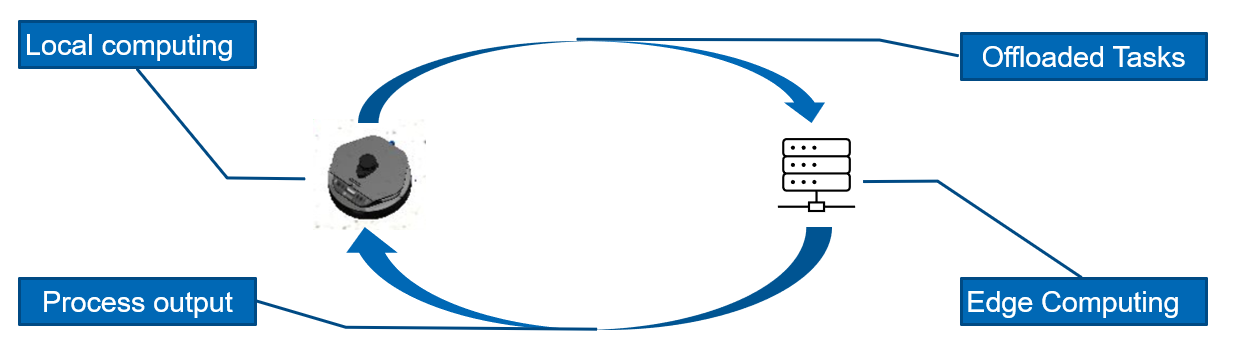
\includegraphics[width=0.8\linewidth]{figures/setup/amr_offloading.png}
    \caption[Computation offloading between \acrshort{amr} and edge computer]{This figure shows the computation offloading between the \gls{amr} and the edge computer. The \gls{amr} can choose to compute the tasks locally or to offload them to the edge computer. If the \gls{amr} chooses to offload, the edge computer will compute the tasks and send the processed output back to the \gls{amr} via the network} 

    \label{fig:amr_offloading}
\end{figure}

Edge computing as an evolution of cloud computing brings application hosting from data centers down to the edge of the network, where the data were initially collected, to achieve low latency and bandwidth efficiency \cite{Lin2019}. For latency-sensitive tasks on \glspl{amr}, such as perception and navigation, Edge computing offers an opportunity to enable the \glspl{amr} with limited resources by offloading costly computation tasks to the edge, while only a small portion of the computation remains on the \gls{amr}'s on-board system. An illustration of computation offloading between the \gls{amr} and the edge computer is shown in \cref{fig:amr_offloading}.

However, depending on the application scenarios, offloading certain tasks from \glspl{amr} to the edge at all times may not be possible, beneficial, or even feasible due to the network's latency, dynamic network changes, and resource availability. \citeauthor*{Baxi2022} \cite{Baxi2022} point out that a simple perception task using an RGB-D camera can cause over 100 ms sensing-to-actuation round-trip latency and over 400 Mbps network bandwidth usage. On the other hand, offloading computational workloads to the edge could also impact the \gls{amr}'s safety, availability as well as on-board resources. The exact influence on the robotic system will depend on the chosen offloading strategy. Therefore, it is necessary to investigate the effects of certain offloading strategies on the \gls{amr}'s safety, availability, and task performance.

% ---------------------------------------------------------------------
\section{Motivation}\label{sec:motivation}
% ---------------------------------------------------------------------

A number of works have investigated the computation offloading strategies as a purely mathematical problem and have proposed different algorithms to solve the problem. However, few of them consider the real application in \glspl{amr}, where the dynamic network changes and onboard resource limitations can affect the performance of the offloading strategies greatly. Therefore, the purpose of this thesis is to investigate the influence of different offloading strategies using actual robotic systems and edge computers in an experimental way.

 With the results from the experiments, this thesis is trying to answer the following research questions: What effects do different offloading strategies have on the specified metrics? Furthermore, this thesis is trying to answer the question: If and how the effects of different offloading strategies vary under different circumstances and if they have any (application-specific) constraints. Finally, this thesis is trying to gain insights if more complex strategies to achieve better results on the metrics. 

 Furthermore, this thesis aims to develop a dynamic offloading strategy that can detect the limitations of the available resources on different systems and can adapt to dynamic changes in network conditions, in order to minimize the execution latency of the offloaded computation task and improve its performance by using edge computers equipped with more computation resources.

% -------------------------------------------------------
\section{Research Methodology}\label{sec:research_methodology}
% -------------------------------------------------------

In order to carry out the experiments, an offloading framework for robot perception is implemented using \gls{ros}2 \cite{Macenski2022} and used to analyze the effects of different offloading strategies. More specifically, this thesis considers a 2D object detection task using the YOLOv5 models, proposed by \citeauthor*{Jocher2022} \cite{Jocher2022}. YOLOv5n, a smaller variant of the perception model, will be deployed on the \gls{amr}'s on-board system, while the edge counterpart uses a more accurate but also a more complex variant, e.g., YOLOv5l. The environment is an industrial warehouse containing different objects as obstacles, which is a common use case for \glspl{amr}. The \gls{amr} is equipped with camera sensors and uses navigation 2, proposed by \citeauthor*{Macenski2020} \cite{Macenski2020}, to navigate through a user-defined route.

First, the baseline strategies are investigated. More specifically, an "edge only" strategy that only offloads to the edge computer, a "robot only" strategy that only uses the \gls{amr}'s onboard system, and a series of strategies that offload to the edge with different ratios are used as the baseline strategies. This step aims to investigate the influence of different offloading strategies on the performance of the perception task and the resource usage of the \gls{amr} and the edge computer as well as the network. Then, a dynamic offloading strategy that makes decisions based on runtime parameters is developed and implemented, such as latency and \gls{amr}'s CPU usage and power consumption. This dynamic offloading strategy aims to minimize latency and improve the performance of the object detection task, inspired by the problem formulation of \citeauthor*{Ning2019} \cite{Ning2019}. Additional constraints subjected to power consumption and network bandwidth are applied to the algorithm. 

In the end, an evaluation framework is implemented based on important metrics of the object detection task performance and the \gls{amr}'s onboard resources. The baseline offloading strategies are first evaluated in simulation to verify the functionalities and the robustness of the offloading framework. Then, the experiments are carried out with an actual robotic system and evaluate the baseline strategies on the defined metrics. With results from the experiments with the baseline strategies, the dynamic offloading strategy is developed and evaluated against the baseline strategies by conducting experiments using Ethernet and Wi-Fi connections. 

\chapter{Background}\label{ch:background}

This chapter describes the fundamental background in different fields that is needed to understand the content of the thesis. An introduction to edge computing is presented in \cref{sec:edge_computing}. In \cref{sec:object_detection}, the \gls{dnn} approach to detect objects in the image is introduced. Finally, the frameworks and software tools used for the implementation of the thesis are introduced in \cref{sec:frameworks_and_tools}.

% ------------------------------------------------
\section{Edge Computing}\label{sec:edge_computing}
% ------------------------------------------------

Edge computing as an evolution of cloud computing brings the application hosting from centralized data centers down to the network edge, closer to the consumers and the data generated by applications, in order to reduce the latency and improve the bandwidth efficiency \cite{Kekki2018}. An illustration of the relation among cloud, edge, and end devices is shown in \cref{fig:mec}

% Figure for edge computing
\begin{figure}
    \centering
    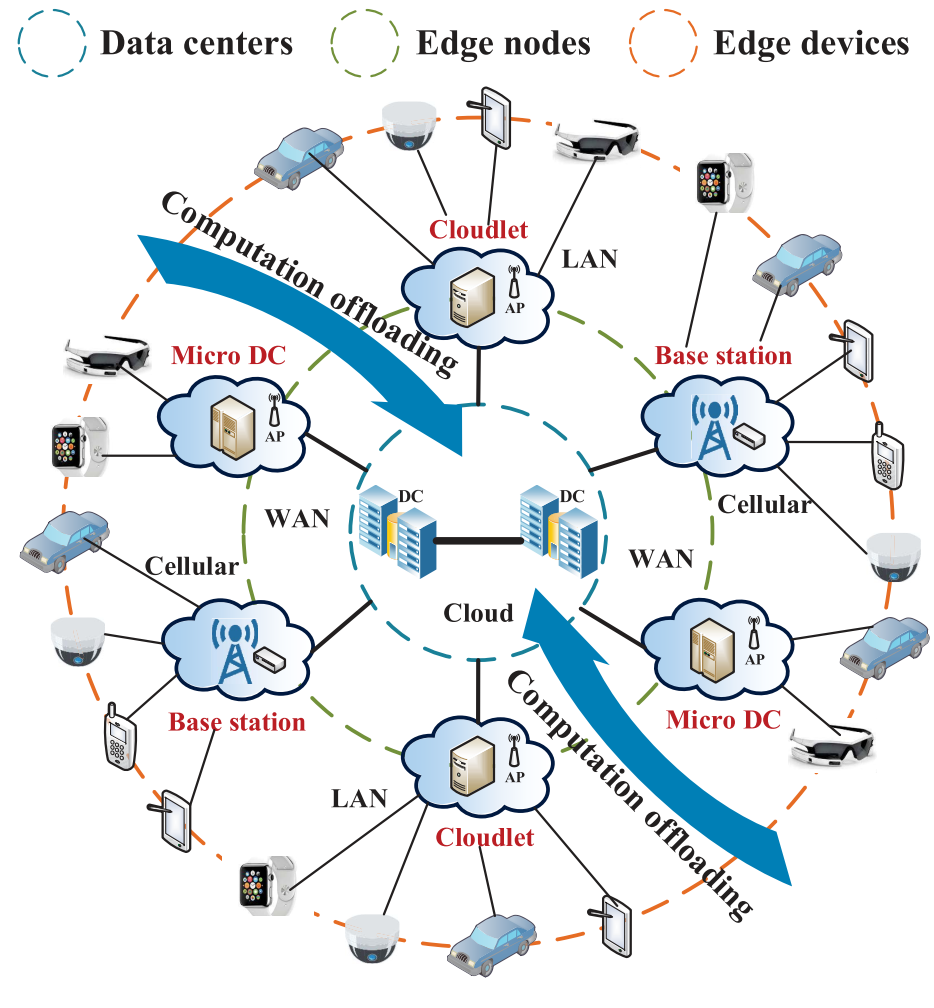
\includegraphics[width=0.6\linewidth]{figures/background/mec.png}
    \caption[A typical three-tier architecture of edge computing with the flow of computation offloading]{A typical three-tier architecture of edge computing with the flow of computation offloading \cite{Lin2019}}
    \label{fig:mec}
\end{figure}

\subsection{Development of edge computing}

Over the last two decades, cloud computing starts to its power in industry, business, and daily life by leveraging powerful infrastructures, such as remote data centers, to augment the computation capabilities of less powerful devices \cite{Lin2019}. Especially with the booming of mobile devices, e.g., smartphones, \gls{mcc}, as the integration of cloud computing and mobile computing, has become recognized as the new generation of computing. However, cloud computing cannot satisfy the latency requirements for time-sensitive tasks. As a result, many efforts have gone into reducing the latency by placing the computing units closer to the end devices. 

To leverage the \gls{wan} delays, jitters, congestion, and failures, \citeauthor*{Satyanarayanan2009} \cite{Satyanarayanan2009} first used \glspl{vm} to instantiate customized service on a nearby "cloudlet", which is a resource-abundant computer or cluster of computers placed at the edge of the Internet as a proof of concept for edge computing. Later on, \citeauthor*{Bonomi2012} \cite{Bonomi2012} introduced fog computing, which allows the end devices to use both edge and cloud computing and defines the connection between the end devices, the edge, and the cloud. In recent years, as an effort to standardize edge computing, ETSI \cite{Kekki2018} announced the \gls{mec} focusing on integrating edge computing with \gls{ran}, especially with 5G network. On the other hand, various companies, including Intel, founded the OpenFog Consortium and introduced the OpenFog as an open architectural framework for fog computing. Then, as a reconciliation of the two standards, ETSI and OpenFog consortium start to collaborate on the application of edge and fog computing. Another approach is the \gls{tsn} \cite{Satka2023}. With a focus on reducing network latency and jitters, \gls{tsn} was initially proposed as a standard for wired communication. However, in recent years, researchers have also gone into the \gls{tsn}-5G integration to achieve \glspl{kpi} in network latency and jitters. 

In the industrial domain, \glspl{iot} supported by Industrial 4.0 have been a key enabler for industrial automation. Therefore, Intel published the edge infrastructure handbook providing ready-to-deploy time-sensitive solutions for \gls{iot} applications \cite{intel-edge-2021}. 

\subsection{Edge robotics}

Robots run different algorithms on their onboard system, such as perception, \gls{slam}, navigation, and path planning. However, the robotic onboard resources are usually limited due to cost and spatial reasons. Offloading some of the computation to the edge can alleviate the workload of the robot's onboard system. This approach, sometimes also called edge robotics, is an ideal use case for edge computing. 

Many works have already proven the concept of edge robotics. \citeauthor*{Huang2022} \cite{Huang2022} show that using edge in multi-robot \gls{slam} algorithm reduces the processing latency. \citeauthor*{Sossalla2022} \cite{Sossalla2022} took a step further by offloading navigation, \gls{slam}, and control functionalities to the edge and ensured the network latency and throughput requirements by using a 5G connection. \citeauthor*{Xie2021} \cite{Xie2021} achieved real-time instance segmentation for mobile robots with limited onboard resources. In the works of \citeauthor*{Fu2019} \cite{Fu2019} and \citeauthor*{Tanwani} \cite{Tanwani}, they both show that offloading the object recognition tasks reduces the execution latency and improves the task performance. 

Although edge computation offloading in robotics does show promising results in reducing execution latency and improving task performance, \citeauthor{Saeik2021} \cite{Saeik2021} pointed out that the dynamic network conditions and the resource allocation are still open challenges in edge robotics. This left several open questions of application partitioning, offloading decision-making, and distributed task execution. 

% ----------------------------------------------------
\section{Object Detection}\label{sec:object_detection}
% ----------------------------------------------------

Object detection, as an essential part of robotic vision, is one of the algorithms the robot runs on its onboard system. It provides bounding boxes and classification of potential objects in the robot's view. In the last two decades, object detection has undergone a paradigm shift from statistical classifiers using hand-crafted features to \gls{dnn} using general-purpose learning procedures and large datasets \cite{RuizdelSolar2018}. \gls{dl}-based methods not only improve the performance of object detection but also increase the computation workload of the robotic system, making it harder to achieve real-time object detection on the robot with complex \gls{dnn} models. Therefore, edge robotics, as a method to alleviate the computation workload of the robot's onboard system, can help achieve real-time execution. 

\subsection{DNN-based object detection}

% short introduction of object detection using neural network
State-of-the-art object detection methods usually consist of a backbone, a neck, and a head, as shown in \cref{fig:object_detector}. The backbone is usually made up of pre-trained \gls{cnn} layers that are used for feature extraction, such as VGG16 \cite{Simonyan2015} and ResNet-50 \cite{He2016}. The neck usually consists of some layers used to collect feature maps from different stages. Finally, the head is responsible for predicting bounding boxes and classes of objects. 

% Figure for object detection algorithm architecture
\begin{figure}
    \centering
    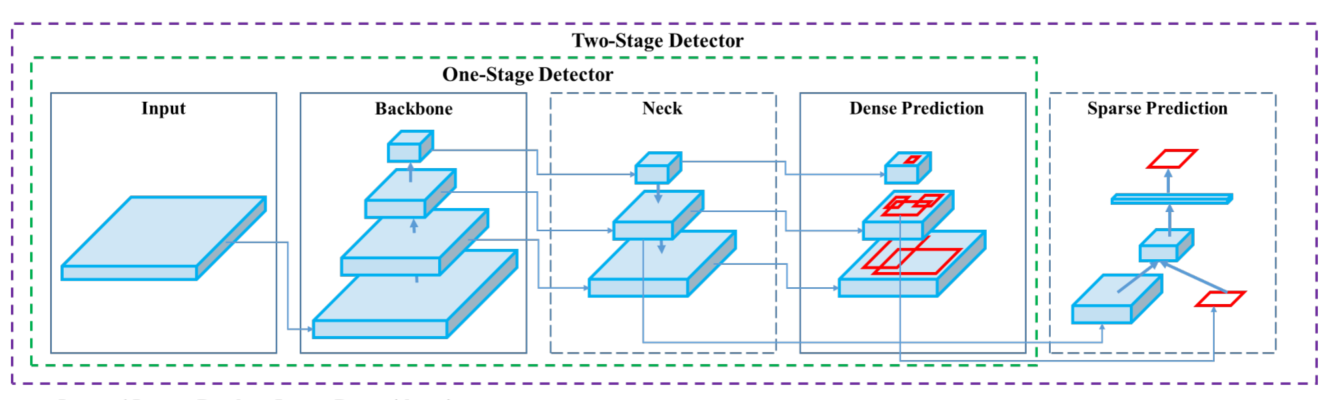
\includegraphics[width=\linewidth]{figures/background/object_detector.png}
    \caption[Architecture of object detection algorithms]{Architecture of object detection algorithms \cite{Bochkovskiy2020}}
    \label{fig:object_detector}
\end{figure}

As shown in \cref{fig:object_detector}, the object detection algorithms can be divided into two categories based on the structure of the head: one-stage detector and two-stage detector. Two-stage detectors, such as Faster R-CNN \cite{Ren2015} and Mask-RCNN \cite{He2017}, have a \gls{rpn} that generates proposals for \gls{roi}. Then, the regressor and classifier detect a bounding box and a class for that \gls{roi}. On the other hand, one-stage detectors, such as SSD \cite{Liu2016} and YOLO \cite{Redmon2016}, have only one network to do both. Benefiting from the simple structure of the head, one-stage detectors are faster but usually come with a trade-off of slight precision detection. However, thanks to their faster inference time, the one-stage detectors can satisfy the real-time requirements of robot vision.

With the development of \gls{dl} algorithms, \gls{dl} frameworks have also undergone major development in the last decade. Frameworks, such as TensorFlow \cite{MartinAbadi2015} and \gls{pytorch} \cite{Paszke2019}, have already been the de facto standards for implementing and training the \gls{dnn}. Moreover, toolkits like \gls{openvino} \cite{Demidovskij2019} can optimize a \gls{dnn} and deploy it on Intel hardware.

\subsection{YOLOv5}

% Introduce the single-stage object detection of YOLO
% Specify how has yolov5 developed
The \gls{yolo} architecture \cite{Redmon2016} as a one-stage detector uses one network to generate the proposals for \gls{roi} and compute regression and classification of objects by dividing the image into many grids and generating detection relative to the center of the grid. This is also known as the anchor-based detector. With the initial success, the \gls{yolo} architecture has also undergone a fruitful development. As of the time of the works of this thesis, \gls{yolo}v5 \cite{Jocher2022} is the current state-of-the-art algorithm for one-stage object detections. 

\gls{yolo}v5 also provides models of various sizes with different object detection performances and inference times. This is easy for deploying them on different platforms. For example, since the robot's onboard system has limited resources, it can use a simple model like the \gls{yolo}v5n. For the edge, complex models, such as \gls{yolo}v5l and \gls{yolo}v5x, can be used. Furthermore, \gls{yolo}v5 can be easily deployed with \gls{pytorch}, which supports Nvidia GPU deployment via CUDA toolkit. 


% ------------------------------------------------------------
\section{Frameworks and Tools}\label{sec:frameworks_and_tools}
% ------------------------------------------------------------

This section introduces the frameworks and software tools that are used during the implementation of the work of this thesis. 

\subsection{Robot Operating System}

% First paragraph as an overview of ROS
\gls{ros} is an open-source robotic operation system, proposed by \citeauthor*{Quigley2009} \cite{Quigley2009}. As described by the author himself, \gls{ros} is not an operating system in the traditional sense, but rather a structured communication layer above the host operating systems. Nevertheless, the emergence of the \gls{ros} has propelled the advancement of robotics immensely for research and commercial applications. However, \gls{ros} starts to show limitations because of its research foundations when its commercial usage transitioned into products \cite{Macenski2022}. Therefore, a redesigned \gls{ros}2 is introduced by \citeauthor*{Macenski2022} \cite{Macenski2022} to tackle the challenges, such as security, reliability, and scalability.

% Second paragraph introducing the difference between ros 1 and ros2
The redesigned \gls{ros}2 differentiates itself from the original \gls{ros} (or \gls{ros}1) in three aspects. Foremost, \gls{ros}2 uses \gls{dds} as its communication layer, unlike \gls{ros}1, which supports \gls{tcp} communication. Instead, \gls{dds} uses the \gls{rtps} protocol, which is built on \gls{udp} \cite{OMG2021}. \gls{ros}2 can benefit from this when the network is lousy, such as wireless communications. Furthermore, using \gls{dds} allows \gls{ros}2 to get rid of the master in \gls{ros}1, since \gls{dds} allows multi-cast and discovery.  Second, unlike \gls{ros}1 where the \gls{python} library "rospy" and the C++ library "roscpp" are written separately in their own language, \gls{ros}2 has a common library written in C language "rcl" on which both the \gls{python} language and the C++ language depend. Therefore, the performance of the two libraries is more consistent in \gls{ros}2.

% Figure for ros communication patterns
\begin{figure}
    \centering
    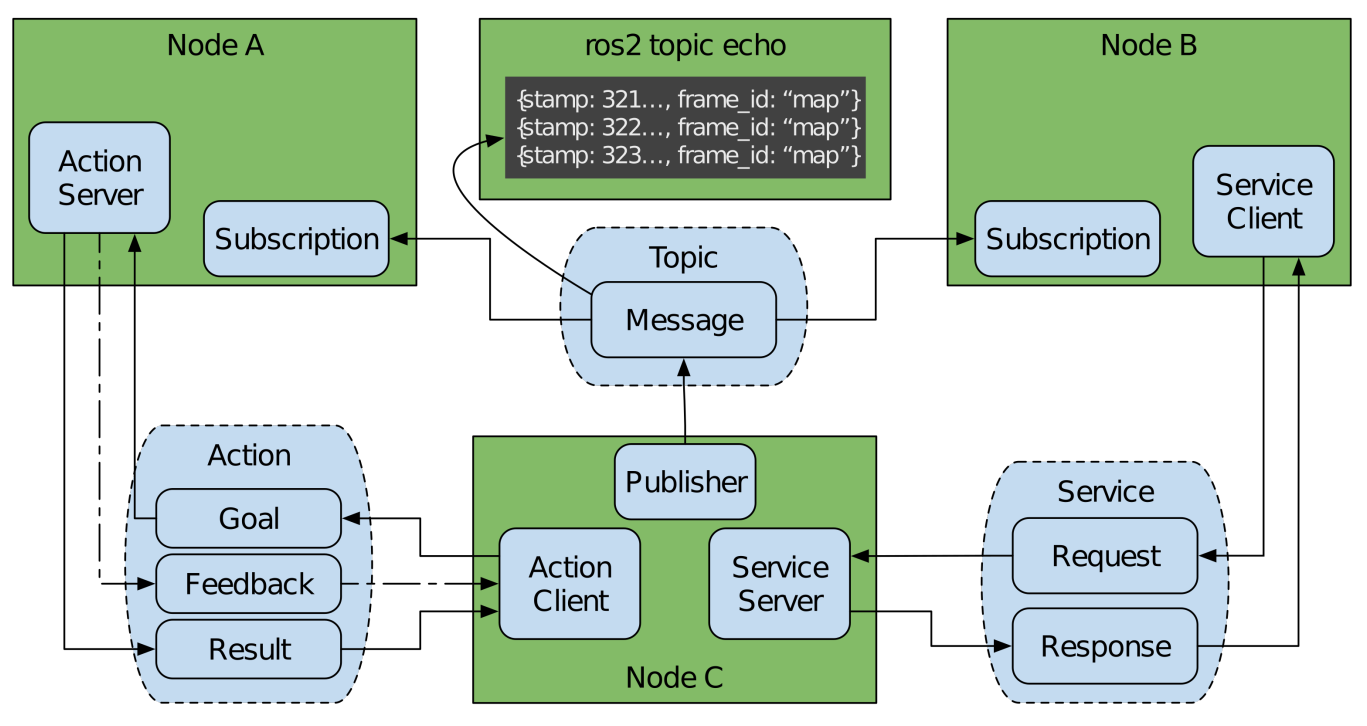
\includegraphics[width=\linewidth]{figures/background/ros2_node_interfaces.png}
    \caption[Communication patterns between \gls{ros}2 nodes]{Communication patterns between \gls{ros}2 nodes \cite{Macenski2022}}
    \label{fig:communication_patterns} 
\end{figure}

% Third paragraph introducing essential topics of ros1 and ros2
\gls{ros} provides a standardized abstraction of communication for robotic applications over multiple machines. This is ideal for use cases like cloud robotics and edge robotics. \gls{ros} provides three communication patterns: topics, services, and actions. A typical \gls{ros}2 application can be illustrated in \cref{fig:communication_patterns}. A \gls{ros} node is responsible for a single, module purpose, such as controlling the camera and doing image processing \cite{ROSGalactic2021} Each node can send and receive data to other nodes via the three communication patterns. The most common pattern is topics. The \gls{ros} nodes communicate by publishing and subscribing to messages on topics. Depending on what information needs to be communicated between the \gls{ros} nodes, the messages use the defined type. With the publish-subscribe pattern, the topics allow many-to-one, one-to-many. as well as many-to-many communication. The services provide a request-response communication. Clients submit requests to the service server, which processes the request and sends a response back to the client asynchronously. Actions provide goal-oriented and asynchronous communication interfaces with a request, response, and periodic feedback. This communication pattern is normally suitable for long-term complex tasks, such as navigation. Other than the communication patterns, the \gls{ros} node can also be configured via the \gls{ros} parameters at startup or during the runtime without changing the code. A \gls{ros} parameter usually needs to be first declared and then used somewhere in the \gls{ros} node. 

Since \gls{ros}2 galactic is the state-of-the-art during the work of this thesis, the name "\gls{ros}" refers to \gls{ros}2 galactic for the rest of the thesis unless specified otherwise. 

\subsection{Gazebo Simulation}

% First paragraph as an overview of Gazebo simulation

\gls{gazebo} is an open-source 3D simulator for robotics. It integrates a physics engine and a rendering engine, and support code for sensor simulation and actuator control \cite{GazeboWiki}. Therefore, the camera sensor can generate realistic RGB images from the simulation. The \gls{gazebo} simulation has undergone a series of name changes during its development, as shown in \cref{fig:gazebo_development}. The original \gls{gazebo}, also now known as \gls{gazebo} classic, is discontinued after the last generation released in 2020. The ignition name is initially used for another approach to differentiate itself from the original \gls{gazebo}, i.e., \gls{gazebo} classic, is changed back to \gls{gazebo} again in 2022 for the current state-of-the-art \gls{gazebo} garden. However, since this thesis uses Gazebo Fortress, due to dependency issues with \gls{ros}, the name \gls{gazebo} refers to \gls{gazebo} fortress for the rest of the thesis for simplicity. 

% Figure for gazebo development
\begin{figure}
    \centering
    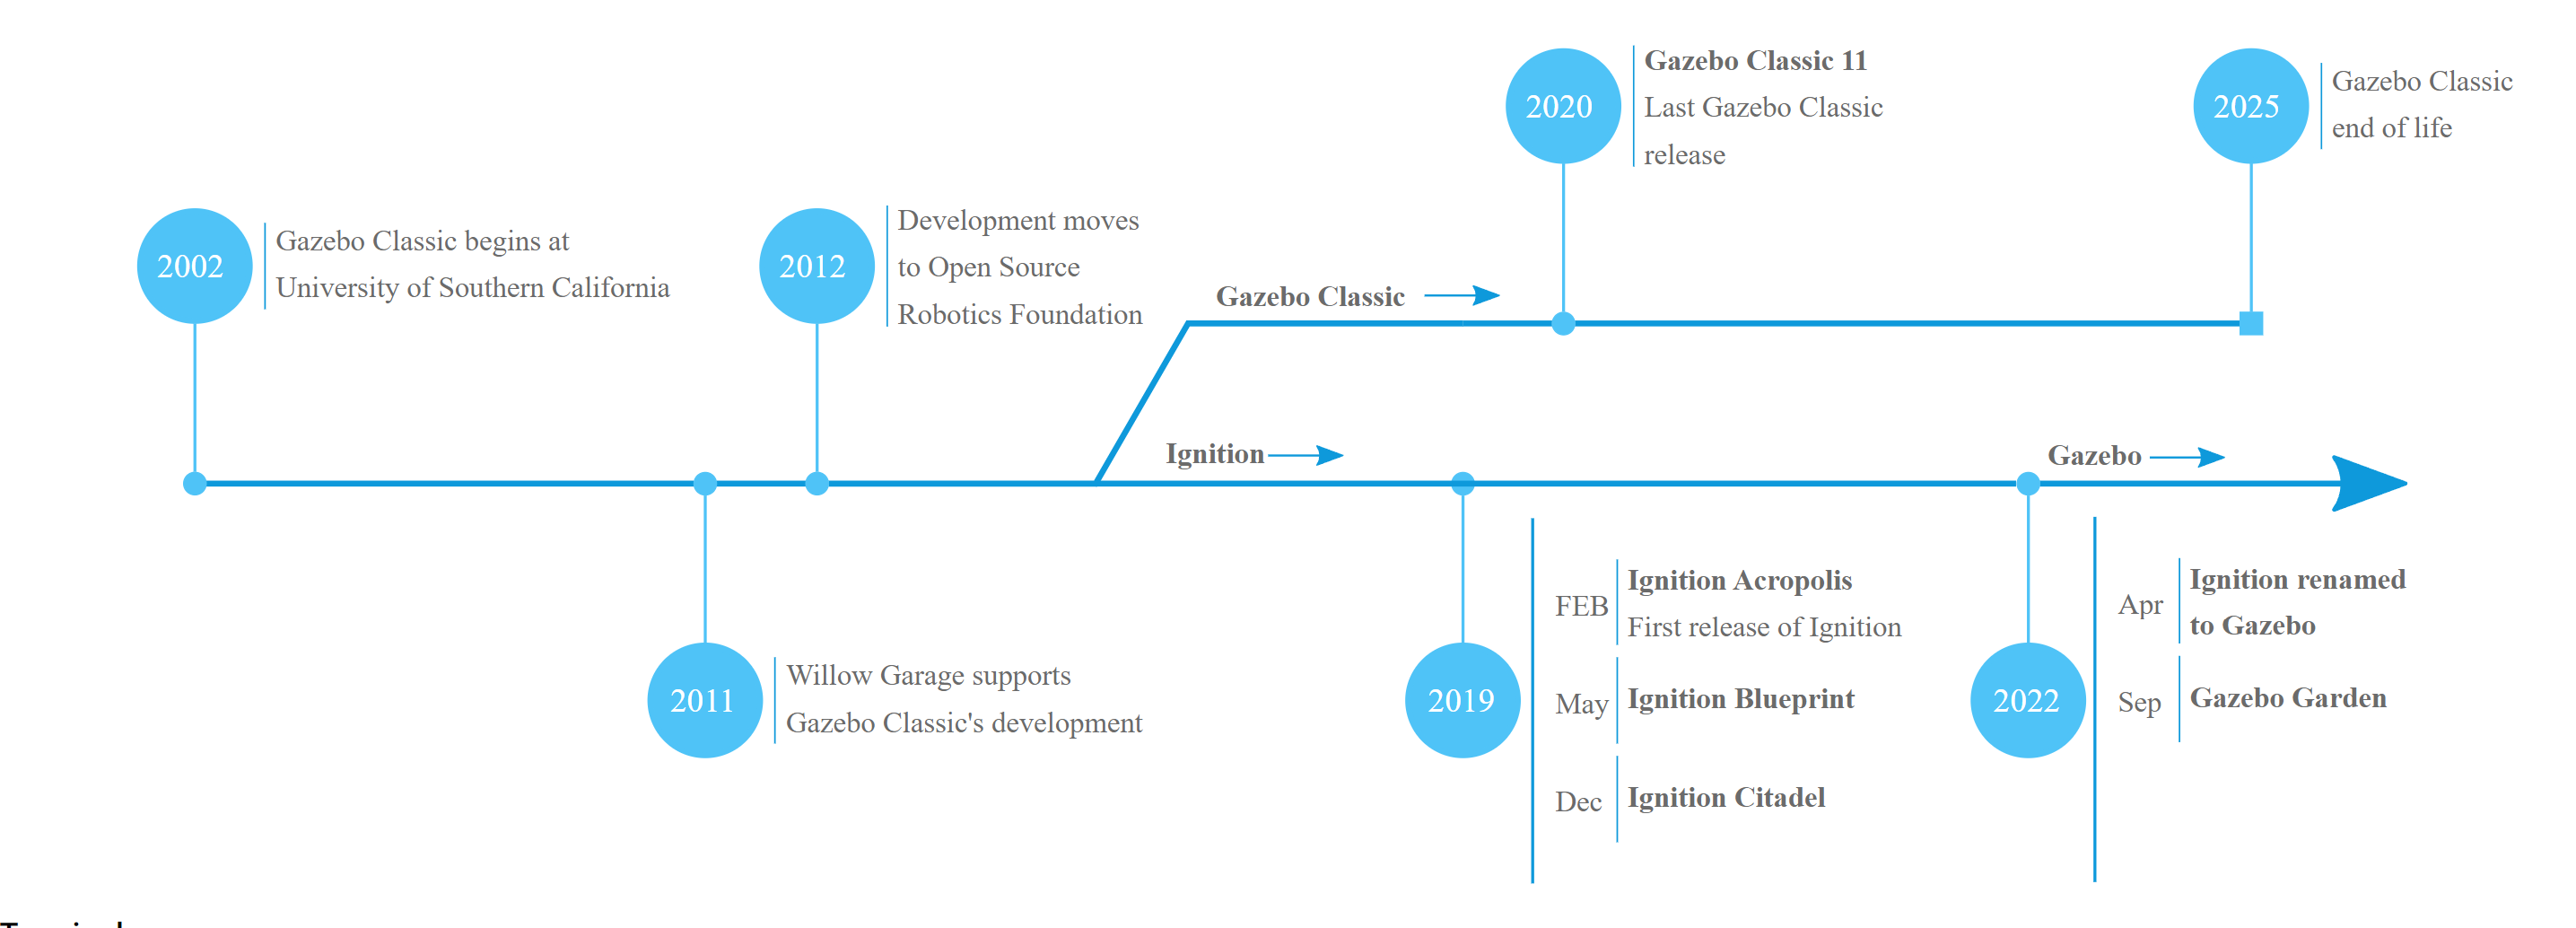
\includegraphics[width=\linewidth]{figures/background/gazebo_development.png}
    \caption{The development of \gls{gazebo} simulation \cite{GazeboSim}} 
    \label{fig:gazebo_development}
\end{figure}

In \gls{gazebo}, the simulation scenarios are implemented as world files and model files, which are written in \gls{sdf} \cite{SDFormat}. The \gls{gazebo} loads the world file on startup and it can load the model files either on startup or during runtime on demand. The \gls{gazebo} client runs a user interface for the server. Camera sensors and bounding box cameras sensors can generate RGB image stream and bounding boxes during simulations. The messages are published in protobuf format and they can be bridged to \gls{ros} messages with \gls{ros}-\gls{gazebo} bridge \cite{GazeboSim}. 

% Second paragraph introduce the development of Gazeob (Classic -> Ign -> Gz)

% Third paragraph introduce how a scenario is implemented in gazebo and what does the gazebo output

\subsection{Network policies}

\gls{netem} is an enhancement of the Linux traffic control facilities that allow one to add characteristics to packets outgoing from a selected network interface \cite{tc-netem}. It can add delay packet loss, duplication, as well as rate. An outgoing policy can be set up for network interface "eth0" as follows: 

\begin{verbatim}
    tc qdisc add dev eth0 root netem delay 100ms loss 10% rate 160Mbit
\end{verbatim}

In this example, the \gls{netem} set the outgoing policy of the network interface "eth0" to 100 ms delay, 10\% packet loss and 160 Mbps bandwidth. However, it is worth noticing that \gls{netem} can only set up outgoing policies. For incoming policies, a \gls{ifb} device needs to be set up and all traffic needs to be redirected to the new network interface. Then, the \gls{netem} can be used to modify the outgoing policies of the \gls{ifb} network interface, which will act as the incoming policies of the original network interface.

\chapter{Related Work}\label{ch:related_works}

A plethora of research has investigated offloading strategies of edge computing. Offloading strategies decide when and how the \glspl{amr} should offload the computation tasks to the edge. They can be mainly divided into three categories: optimization approaches, game theory approaches, and learning-based approaches. This chapter gives a short introduction to these approaches. 

% Old structure here
% --------------------------------------------------------------
% \section{Task Offloading Goals}\label{sec:task_offloading_goals}

% % Introduce why the robot offloads to edge

% \subsection{Performance improvement}

% % First paragraph, reduce latency

% % Second paragraph, improve computation capabilities

% \subsection{Resource usage}

% \section{Approaches}\label{sec:approaches}

% \subsection{Optimization approaches}

% \subsection{Game theory approaches}

% \subsection{Learning-based approaches}
% --------------------------------------------------------------

\section{Optimization Approaches}\label{sec:optimization_approaches}

Optimization approaches formulate the computation offloading problem as an optimization problem with the goal to minimize energy consumption and/or execution latency. The multi-robot computation offloading can be usually formulated as an integer linear programming problem. The offloading strategy is derived from the problem solution. 

\citeauthor*{Zhao2015} \cite{Zhao2015} formulate the problem as a joint optimization problem of the radio and computation resources aiming to reduce the overall energy consumption of mobile devices. The energy consumption model consists of two components: energy to transmit data and energy to compute the task locally. \citeauthor*{Zhao2015} also consider task partitioning in computation offloading. In the mathematical model, the computation task can be partitioned and partially offloaded without overhead for partitioning. In the end, \citeauthor*{Zhao2015} propose a heuristic algorithm to find the sub-optimal solution. \citeauthor*{Chen2015} \cite{Chen2015} formulate the problem as a non-convex quadratic program with the goal of minimizing an offloading cost which consists of weighted energy consumption and execution latency. \citeauthor*{Chen2015} solve the problem by applying a semi-definite relaxation and a randomization mapping method to the optimization problem. It is worth mentioning that the aforementioned works still focus on the mobile cloud computing paradigm, which only considers the cloud as the destination of computation offloading. However, the approaches are transferable to edge computing. 

With the emergence of edge computation offloading, edge computers can also be used to perform computational tasks. \citeauthor*{Guo2018} \cite{Guo2018} consider the case where the end devices can choose to offload either to centralized data centers or to edge computers. The problem is formulated as an optimization problem with the goal of minimizing energy consumption with a constraint for maximal execution latency. An exhaustive algorithm is proposed to find the optimal solution. \citeauthor*{Ning2019} \cite{Ning2019} consider not only the three computation options but also the computation task partitioning and distribution among the local system, edge computer, and the cloud. Therefore, the problem is formulated as a mixed integer linear programming problem aiming to reduce the execution latency, which also inspired the problem formulation of the work of this thesis. An iterative heuristic algorithm is proposed to solve the problem. 

The formulated optimization problem with a joint optimization goal is, in general, a mixed integer linear programming problem and cannot be solved in polynomial time. Therefore, on the one hand, heuristic algorithms are proposed to find the sub-optimal solution. On the other hand, relaxation is applied to the problem to find the approximate optimal solution. Furthermore, the optimization approaches assume a central decision-making unit that has full knowledge of the entire system. However, with dynamic network conditions and time-sensitive computation tasks, this may not be the case for the edge and the robot. Therefore, an offloading strategy with the ability to adapt to dynamic network changes and satisfy real-time requirements of the computation task is needed. 

\section{Game Theory Approaches}\label{sec:game_theory_approaches}

Unlike the optimization approaches, the game theory approaches formulate the problem as a game where end devices are players of the game. The offloading decision is made by finding an optimum or a \gls{ne} of the game. A \gls{ne} is a group of strategies where no player can profit by modifying his strategy while the other players’ strategies are kept unchanged \cite{Chaari2022}. Therefore, the game theory approaches are intrinsically distributed since the players make their own decisions. 

\citeauthor*{Chen2016} \cite{Chen2016} formulate the distributed computation offloading decision-making problem among mobile device users as a multi-user computation offloading game. The approach aims to minimize a cost function consisting of energy consumption and execution latency. In the end, a distributed computation offloading algorithm is proposed to solve the problem. Furthermore, \citeauthor*{Pham2018} \cite{Pham2018} also consider the scenario where multiple users offload to multiple servers. The problem is formulated as a joint optimization problem with the goal of optimizing the transmit power of the users and the computation resources at the servers. Two distributed matching algorithms are proposed to choose the server and the sub-channel. \citeauthor*{Hong2019} \cite{Hong2019} take another step further by considering the computation offloading routing. The problem is formulated as a multi-hop cooperative computation offloading game. They further proposed a distributed algorithm to attain the \gls{ne} of the game for partitioned and unpartitioned tasks. In addition, \citeauthor*{Xu2020} \cite{Xu2020} investigate how the weight factor in a cost function consisting of different optimization goals affects the overall system performance. 

The game theory approaches allow distributed decision-making. However, the algorithms usually require several iterations for the cost function to converge and reach the \gls{ne}. The communication overhead will increase with the number of end devices. Furthermore, the works lack experiments with real applications and only approach the problem as a purely mathematical problem. 

\section{Learning-based Approaches}\label{sec:learning_based_approaches}

In recent years, \gls{drl} has been used widely for decision-making problems. In edge computation offloading, the offloading strategy can also be modeled as a \gls{dnn}. Different offloading options are treated as the action space. Network conditions and robot onboard resources are considered as the state space. Since the learning-based approaches do not need a model of the system, they are more capable of dealing with dynamic changes in the network. 

\citeauthor*{Huang2019} \cite{Huang2019} train a \gls{dqn} agent to make offloading decisions for multi-users computation offloading. The reward function is formulated to reduce energy consumption and execution latency. \citeauthor*{Lu2020} \cite{Lu2020} take another step further with the \gls{dqn} agent by considering task partitioning for multi-user and multi-server computation offloading problems. The reward function is formulated to improve energy consumption, load balancing, and execution latency. 

Several works from these approaches also demonstrate real application performance. \citeauthor*{Chinchali2019} \cite{Chinchali2019} train a \gls{a2c} agent to perform computation offloading with face recognition algorithm. The agent shows improved performance in accuracy and execution time compared with naive offloading strategies, such as only offloading to the edge, only computing locally, and random offloading. Moreover, \citeauthor*{Penmetcha2021} \cite{Penmetcha2021} offload navigation tasks to the cloud. The trained \gls{dqn} agent is capable of making offloading decisions by considering the data size of the task. Finally, \citeauthor*{Ruggeri2022} \cite{Ruggeri2022} trains a \gls{dqn} agent to make offloading decisions for scene understanding, which is a safety risk evaluation task. The safety risk is reduced compared to naive offloading strategies. 

Learning-based approaches show promising results in dealing with dynamic network changes and can make offloading decisions in a distributed manner. However, the computation of the \gls{dnn} also causes additional execution latency and increases the computation workload of the robot's onboard system. For time-sensitive tasks, such as object detection, the additional execution latency can cause the performance to deteriorate.

In the end, it is also worth noticing that a plethora of literature has already investigated the mathematical problem of computation offloading and various approaches have been proposed to tackle the problem. However, few investigate the influence of different strategies on the robotic system metrics in an experimental way. Therefore, this thesis intends to investigate this problem by implementing an offloading framework and conducting experiments on the influence of different offloading strategies. 
\chapter{Methodology}\label{ch:methodology}

This chapter describes the methodology the thesis adopts to solve the problem. In \cref{sec:system_design}, the system design of the perception offloading is presented and explained. Then, the offloading strategies are described in \cref{sec:offloading_decision}. 

% -----------------------------------------------
\section{System Design}\label{sec:system_design}
% -----------------------------------------------

This thesis designs and implements a perception offloading framework and different offloading strategies in order to carry out the experiments. This section first describes the design for an offloading framework based on perception tasks. Then, different offloading strategies are presented. Finally, this section describes what system states are chosen to represent the state of the perception offloading.

\subsection{Perception offloading}

\begin{figure}[htp]
    \centering
    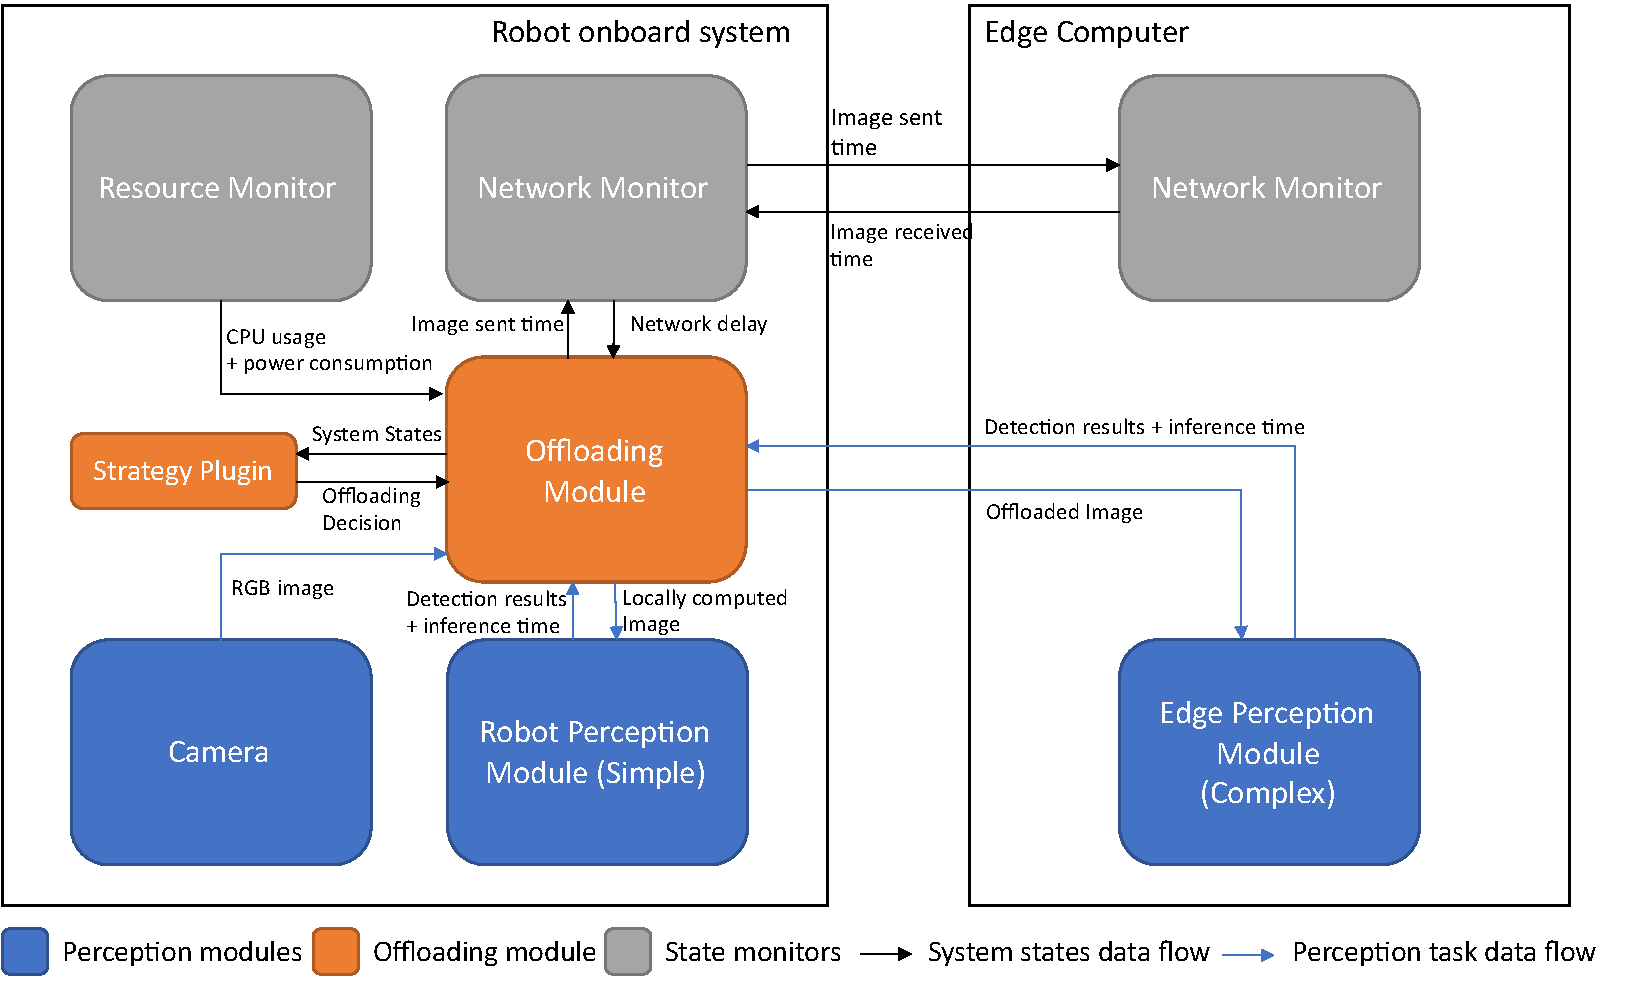
\includegraphics[width=\linewidth]{figures/setup/system_design.pdf}
    \caption[Design of perception offloading framework]{Design of perception offloading framework where the robot and the edge systems are separated by rectangles. Each system consists of different modules that are responsible for different tasks. The orange blocks represent modules related to offloading, while the blue blocks represent modules related to perception tasks. The grey blocks represent modules measuring system states. Arrows show the direction of data flows.}
    \label{fig:perception_offloading_framework}
\end{figure}

The designed offloading framework is illustrated in \cref{fig:perception_offloading_framework}. As shown, this thesis only investigates the scenario where one \gls{amr} offloads the perception task to one edge computer. Therefore, the offloading modules are located solely on the robot's onboard system. To ensure the safety of the robot in case of a complete network connection loss, a perception module is also included on the robot's onboard system. However, since the robot onboard system usually has limited resources, the onboard perception module uses a less computationally expensive object detection model. In contrast, the edge computer has abundant resources. Therefore, it uses a perception module with a more complex model with higher precision. 

% Besides the processed detection, the perception modules also record the inference time used for each detection and return it to the offloading module. Furthermore, a network monitor is set up between the robot and the edge systems to measure the network latency. Finally, a resource monitor is used on the robot's onboard system to measure the onboard resource usage.

To evaluate different offloading strategies, the offloading module adopts a plugin mechanism to load the offloading strategies at startup. The offloading module receives different system states from the state monitors located on the robot's onboard system and on the edge computer. When the offloading module receives an image from the camera, it has to make a decision whether to offload the image to the edge computer or to compute it locally on the robot. Therefore, the offloading module passes the system states to the strategy plugin as run-time parameters and receives the offloading decision. 

In addition to the perception modules and the offloading modules, there are also different state monitors that keep track of the onboard resources of the robot and the network condition between the robot and the edge computer. The network monitor measures the network latency between the robot and the edge computer. The resource monitor monitors CPU usage and energy consumption of the robot's onboard system. Furthermore, the perception modules are also responsible for measuring the inference times of the object detection models and sending them back to the offloading module 

\subsection{System States}

Various system states are considered for the perception offloading. They can be mainly divided into two categories: the onboard resources and the network condition. The network condition is measured by the network delay between the robot's onboard system and the edge computer. The outgoing data of the robot include the offloaded images with their sent times, while the incoming data contain an array of object detection results and the times when the edge computer receives the offloaded images and sends the detection back. The network monitors measure both the outgoing and incoming network delays. The total network delay can be calculated by

\begin{equation}
    t_{network} = t_{network}^{out} + t_{network}^{in}
\end{equation}

where $t_{network}^{out}$ is the network outgoing delay and the $t_{network}^{out}$ is the network outgoing delay. They can be calculated as

\begin{equation*}
    t_{network}^{out} = t_{sent}^{robot} - t_{received}^{edge}
\end{equation*}
\begin{equation*}
    t_{network}^{in} = t_{sent}^{edge} - t_{received}^{robot}
\end{equation*}

For onboard resource usage, the \gls{cpu} usage, the power consumption, and the bandwidth usage are measured. The \gls{cpu} usage and the power consumption can be directly measured with the robot's onboard system. However, the bandwidth usage needs to be calculated with the network IO measurements as follows:

\begin{equation}
    bandwidth = \frac{n_{t_2} - n_{t_1}}{t_2 - t_1} \times 10^{-6} 
\end{equation}

where $n_{t_i}$ represents the number of bytes the network has sent till time $t_i$. The bandwidth is calculated in megabytes per second (MB/s). 

The onboard resource usage represents the availability of the \gls{amr}. If the \gls{cpu} usage is too high, the robot can have no resources left for other tasks performed onboard, such as \gls{slam} and navigation, and cannot operate anymore. Similarly, if the power consumption is too high, the robot needs to be recharged more often. Moreover, if the available bandwidth of the robot network is too small, the robot cannot communicate via the network. Therefore, these measurements are used as system states for making offloading decisions. 

% ----------------------------------------------------------
\section{Offloading Decision}\label{sec:offloading_decision}
% ----------------------------------------------------------

For the offloading module to make offloading decisions, an offloading strategy is needed. In this thesis, several naive strategies are first investigated as baseline strategies. Their influence on various metrics of the system is evaluated. Based on their performance, a dynamic offloading strategy that uses the run-time system states, which are described in \cref{sec:system_design}, is implemented and evaluated against the baseline strategies. 

\subsection{Baseline strategies}

As baselines, this thesis first investigates the scenarios where the robot only computes the object detection task locally on its onboard system or only offloads the task to the edge computer. These two strategies are named the "robot only" strategy and the "edge only" strategy. Then, the thesis continues to investigate the scenarios where the robot offloads a portion of the frames with a fixed ratio. For example, an offloading ratio of 0.2 will allows the offloading module to offload one image to the edge for every five images. The offloading strategies with a fixed offloading ratio can be realized with \cref{alg:ratio_strategy}. The offloading ratio should be a value ranging from 0 to 1. 

\begin{algorithm}[htp]
\caption{Algorithm to offload with a fixed ratio}\label{alg:ratio_strategy}
\begin{algorithmic}[1]
    \Function{RatioStrategy}{$r$} \Comment{where r is the offloading ratio}
        \State $c_1 \gets \, $GetImageCounter()\Comment{Get the counter for the total images received}
        \State $c_2 \gets \, $GetOffloadCounter()\Comment{Get the counter for the images offloaded}
        \State SetImageCounter($c_1 + 1$) \Comment{Add one first to image counter to avoid zero division}
        \If{$c_2 / c_1 \ge r$}
            \State return false \Comment{Compute locally}
        \Else
            \State SetOffloadCounter($c_2 + 1$)
            \State return true \Comment{Offload to edge computer}
        \EndIf
    \EndFunction
\end{algorithmic}
\end{algorithm}

With results from the experiments on baseline offloading strategies, this thesis intends to find the limits of the system and analyze its behavior. More specifically, the experiments and evaluation with the baseline strategies intend to investigate the question that under what circumstances the performance of the perception performance starts to deteriorate and offloading the perception tasks is no longer beneficial for the robot. With the results, this thesis then develops and implements a dynamic offloading strategy that uses run-time system states to make offloading decisions. 

\subsection{Dynamic offloading}

The dynamic offloading strategy aims to adapt to the changes in robot and edge systems as well as in network conditions.  For the one-robot-one-edge scenario, this thesis uses a simplified version of the offloading strategy proposed by \citeauthor*{Ning2019} \cite{Ning2019} with the goal of minimizing the execution latency and improving the average precision of the object detection task. Moreover, this dynamic offloading strategy is subjected to the constraints of other system states. In this thesis, we consider two run-time system states as constraints: \gls{amr}'s \gls{cpu} usage and the network bandwidth. The problem can be formulated as a constraint optimization problem as follow:

\begin{equation}
    \min_{(\alpha, \beta)} \: t_{latency} = t_{inference} + t_{network}
\end{equation}

with

\begin{equation*}
    t_{inference} = \alpha t_{inference}^{L} + \beta t_{inference}^{E}
\end{equation*}
\begin{equation*}
    t_{network} = \alpha t_{network}^{L} + \beta t_{network}^{E}
\end{equation*}

s.t.

\begin{equation*}
    \alpha + \beta = 1
\end{equation*}

\begin{align*}
    & \alpha = \begin{cases}
        1, & \text{if the task is processed locally} \\
        0, & \text{else.}
    \end{cases} \\
    & \beta = \begin{cases}
        1, & \text{if the task is processed by the edge computer} \\
        0, & \text{else.}
    \end{cases}
\end{align*}

where the $t_{latency}$ represents the overall execution latency of the object detection task and $t_{inference}$ and $t_{network}$ represent the inference time and the network delay correspondingly. The execution latency is also called the \acrlong{rtt}. It measures the time for a round trip from the offloading module to the perception modules either located on the robot's onboard system or on the edge computer. 

In addition to the execution latency, the offloading decision is also subjected to the \gls{amr}'s \gls{cpu} usage and the network throughput. If the \gls{cpu} usage exceeds a certain value, the \gls{amr} only offloads to the edge. Similarly, the \gls{amr} only computes the task locally if the network throughput exceeds the threshold. These constraints ensure that the \gls{amr} and the network are capable of finishing the task at all. The decision-making strategy can be implemented as \cref{alg:decision_making_strategy}.

\begin{algorithm}[htp]
\caption{Algorithm to offload with dynamic parameters}\label{alg:decision_making_strategy}
\begin{algorithmic}[1]
    \Function{DecisionMakingStrategy}{$params$}\Comment{run-time parameters: $params$}
        \State $cpu_{max} \gets$ GetMaxCPULevel()
        \If{params['cpu\textunderscore usage'] $\geq cpu_{max}$} 
            \State return true \Comment{Offload if CPU usage exceeds limit}
        \EndIf
        \State $throughput_{max} \gets$ GetMaxThroughput()
        \If{params['bandwidth'] $\geq throughput_{max}$}
            \State return false \Comment{Compute locally if bandwidth usage exceeds limit}
        \EndIf
        
        \State $latency_{robot} \gets $ params['robot\textunderscore inference\textunderscore time'] + params['robot\textunderscore network\textunderscore delay']
        \State $latency_{edge} \gets $ params['edge\textunderscore inference\textunderscore time'] + params['edge\textunderscore network\textunderscore delay']
        \If{$latency_{robot} \geq latency_{edge}$}
            \State return true \Comment{Offload if edge RTT is higher}
        \Else
            \State return false \Comment{Compute locally if edge RTT is higher}
        \EndIf
    \EndFunction
\end{algorithmic}
\end{algorithm}

\chapter{Implementation}\label{ch:implementation}

This chapter focuses on the implementation of the offloading frameworks designed in \cref{ch:methodology}. In \cref{sec:offloading_framework}, the implementation of the offloading framework is described. In \cref{sec:state_monitors}, it describes how the system states are measured for the robot and edge. 

% ------------------------------------------------------------
\section{Offloading Framework}\label{sec:offloading_framework}
% ------------------------------------------------------------

The offloading framework is implemented with \gls{ros}. Different modules are implemented as \gls{ros} nodes and the communication between the nodes uses \gls{ros} topics, as illustrated in \cref{}

% Template for single figure
\begin{figure}
    \centering
    \includegraphics[width=\linewidth]{setup}  % TODO: change here
    \caption{TODO: Change the caption here}  % TODO: change here
    \label{fig:example_figure}  % TODO: change here
\end{figure}

\subsection{Offloading Module}

% Add how is offloading module is implemented in ROS

\subsection{Perception Module}

% discuss the choice of synchronous inference and asynchronous inference. Also defend not retraining the model.

% TODO: add specifications for pytorch perception, e.g., IoU threshold etc. 

% TODO: find the quote on the edge computers
In general, an offloading task can be any computationally intensive algorithms an \gls{amr} is required to run, such as perception, navigation, \gls{slam}, path planning, etc. This thesis chooses an object detection task as an example because an object detection task can have a significant performance difference between the robot's onboard system and the edge computer, which corresponds to the usage scenario of the edge offloading. An \gls{amr} is usually equipped with a simple onboard system with only access to \gls{cpu}, while edge computers are usually cloudlets and data centers on-premise with access to \gls{gpu}. As mentioned in (TODO: add a reference here), the \glspl{amr} use primarily \glspl{dnn} to detect objects. With frameworks like PyTorch that can make use of the \gls{gpu}, the performance difference between \gls{amr}'s onboard system and the edge computer is immense. Therefore, this thesis chooses object detection as an example for offloading tasks. 

% TODO: fill in the real value
\begin{table}[htb]%
    \centering%
    \begin{tabular}{lccccc}
        \toprule
        Model &                     YOLOv5n &   YOLOv5s &   YOLOv5m &   YOLOv5l &   YOLOv5x \\
        \midrule
        Robot inference time &      50.88 ms &  115.75 ms & 240.06 ms & 464.22 ms & 821.93 ms  \\
        Edge inference time &       8.87 ms &   11.51 ms &  20.35 ms &  31.18 ms &  52.55 ms  \\
        Model size &                4 MB &      14 MB &     41 MB &     89 MB &     166 MB    \\
        \gls{map} &                 45.7\% &    56.8\% &    64.1\% &    67.3\% &    68.9\%  \\
        \bottomrule
    \end{tabular}
    \caption{Inference times of different YOLOv5 models on \gls{amr}'s onboard system and edge computer}
    \label{tab:inference_time}%
\end{table}

% TODO: ask if it's okay to list the hardware specification
% TODO: better phrasing
In order to adapt to the performance difference between the \gls{amr}'s onboard system and the edge computer, the perception module should have two models available for object detection: a lightweight model that runs on the onboard system and a more complex model that runs on the edge computer. \gls{yolov5} provides a series of models with different complexities. To find appropriate models for the onboard system and the edge computer, this thesis investigates the inference times of different models on different machines, which can be taken from \cref{tab:inference_time}. To simulate the computation capability discrepancy between the two systems, this experiment uses a \gls{nuc} equipped only with an Intel(R) Core(TM) i3-8109U \gls{cpu}. On the other hand, the edge computer is equipped with an Intel(R) Core(TM) i9-7900X \gls{cpu} and a Nvidia GeForce GTX 1060 6GB \gls{gpu}. The models are deployed with \gls{pytorch} and output an array of bounding box detection. The inference time is measured between the time when the \gls{yolov5} receives the image and the time when the perception node outputs an array of bounding box detection. This includes the time for image pre-processing and the time of results post-processing. Furthermore, the image input for the offloading module has a frame rate around 25 frames per second. To achieve real-time, it is necessary that the inference time does not exceed 100 ms (\textbf{\textit{maybe phrase it better here}}). Longer inference time also causes the actual precision of the object detection to deteriorate, which will be discussed in (TODO: add a reference here). The model sizes and the \gls{map} data are taken from the documentation from \citeauthor*{Jocher2022} \cite{Jocher2022}. The \gls{map} data are evaluated on \gls{coco} val2017 \cite{Lin2014}. As a compromise between the inference time and the performance, this thesis chooses to deploy \gls{yolov5}n on the \gls{amr}'s onboard system and \gls{yolov5}l on the edge computer. 

To delimit, the object detection models in use are pre-trained and not re-trained with custom data from the simulation. This thesis intends to investigate different offloading strategies and generating custom data sets and re-training the models are laborious tasks. Therefore, a re-training of the models is beyond the scope of this thesis. \citeauthor*{Jocher2022} \cite{Jocher2022} state that the all pre-trained models are trained on \gls{coco} data-sets for 300 epochs with default settings. Moreover, this thesis only considers human obstacles, which is a detection class in \gls{coco} data sets. Therefore, the pre-trained models can provide comparability between different offloading strategies on different machines. Furthermore, re-training of the models is dependent on the quality and the size of the custom data sets. An improper re-training can introduce additional errors or over-fitting of the models and thus undermine the comparability. 

% ------------------------------------------------
\section{State Monitors}\label{sec:state_monitors}
% ------------------------------------------------

To evaluate different offloading strategies, this thesis needs to get access to the system states, such as the \gls{cpu} usage, energy consumption, and network bandwidth. Various modules are implemented to measure them. 
The measurements from these modules are recorded for evaluation and also used for dynamic strategies that make decisions based on the run-time states of the system. However, in simulation experiments, the virtualization of the \gls{amr}'s onboard system and the edge computer is realized by the \gls{docker} containers. In contrast, different physical computers are used in real-robot experiments. This difference in the system virtualization affects how the system states are measured. 

\subsection{Network}

\subsection{Onboard resources}
For simulation experiments, \gls{docker} provides the containerized system virtualization and virtual network interfaces. \citeauthor*{Ruggeri2022} \cite{Ruggeri2022} proposes that the network bandwidth in use can be measured with the network throughput. The network throughput and \gls{cpu} usage can be measured with the statistics of the \gls{docker} containers, which is a functionality provided by \gls{docker}. Alternatively, the system states of containers can be monitored using \gls{cadvisor}. For real-robot experiments, the \gls{cpu} usage and the network throughput are measured separately on different machines using \gls{psutil} tools. In the case of Intel \glspl{cpu}, the power consumption can be measured with \gls{rapl} provided by \gls{linux} kernel Power Capping Framework. The measurements of CPU usage, network throughput, and power consumption are provided by the "system status" Python package of the code base of \gls{amsrl}. \citeauthor*{Xie2021} \cite{Xie2021} propose that the execution latency of the offloading task consists of two components: the network delay and the inference time. The network delay measures the time needed for transferring the data from the offloading module to the perception module, while the inference time measures the time the perception module needs to process the inference, including the time for image pre-processing and result post-processing. The execution latency is measured with timers residing in the offloading module and the perception module. The timers record the time stamps to critical time points in the transfer and inference process and calculate the time difference. Then, the data are published to a \gls{ros} topic and can be accessed by other subscribers. 

% TODO: not sure if this paragraph is necessary
Since it is assumed that the edge computer has abundant resources, the system states of the edge computer are not measured and are not taken into consideration during the decision-making and evaluation process. Furthermore, even though this thesis only investigates the single-robot single-edge scenario, the available resources from the edge computers can be affected by numerous factors in real-world applications, such as the number of edge computers, the number of \glspl{amr}, and other processes running the edge computers. In addition, with more powerful hardware and easy access to a power supply, the edge computer consumes more energy and computation resources for the same task than the \gls{amr}'s onboard system. Therefore, it is pointless to compare the consumption of the resources between two systems with na\"{i}vet\'{e}. In contrast, the network connection between the \gls{amr} and the edge computer is fragile and prone to disturbance. Therefore, this thesis only considers the system states of the \gls{amr}'s onboard system and the network condition between the \gls{amr} and the edge computer. 

\chapter{Experiments}\label{ch:experiment}

\section{Simulated scenario}

To run experiments both in simulation and on real robots, this thesis implements a simulated scenario of a factory warehouse with one \gls{amr} and obstacles. The simulation is recorded and replayed for each experiment run to reduce the computation overhead of the simulation and to make the experiment repeatable. Furthermore, in order to compare the results from the simulation and the real robot, the simulation recording is used as input for both experiments under the same replay settings. 

\subsection{Environment}

% include a bird-view shot for the simulation with warehouse, robot, and human obstacles in the view.
The scenario simulates a modern-day factory warehouse, illustrated in (refer to the figure here). The simulated scenario is implemented in \gls{gazebo} with the help of a software package called "scenario execution", which the author implemented during his work at Intel Labs. The scenario consists of a factory warehouse environment and static obstacles, such as humans, boxes, shelves, and pallets, which are common obstacles in a factory warehouse. Since the object detection models are pre-trained with \gls{coco} data sets, which do not contain many of the static obstacles. The evaluation for the \gls{map} of the object detection task is restricted only to detecting human obstacles. To clarify, the object detection models still detect all of the classes that are defined in the \gls{coco} data sets. However, only the human class is taken into consideration when calculating the \gls{map} metric during the evaluation. Since the performance difference among different \gls{yolov5} models are negligible when the scene is too simple, this thesis includes ten human obstacles in the simulated scenario to increase the complexity of the object detection task. Moreover, some human obstacles are occluded by other obstacles in the scenario. Detecting occluded objects has been proven to be a challenging task in object detection. 

\begin{figure}
    \centering
    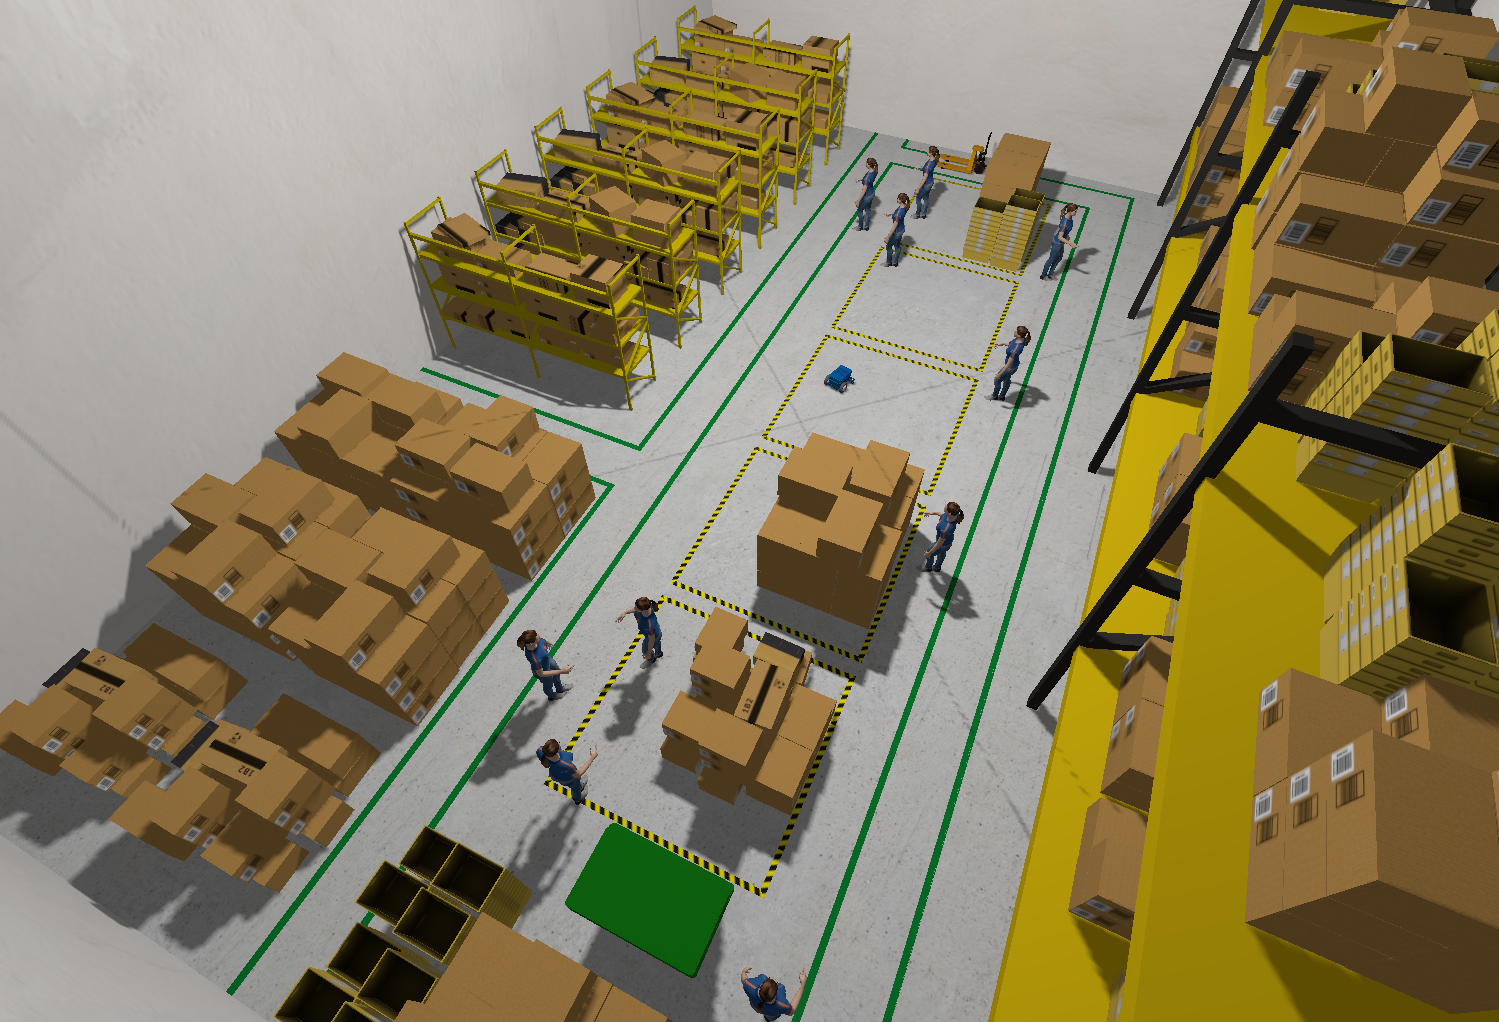
\includegraphics[width=\linewidth]{figures/sim/bird_view.png}
    \caption{Bird view of the simulated scenario}
    \label{fig:bird_view_scenario}
\end{figure}

\subsection{Robot}

The \gls{amr} is implemented as a dynamic obstacle in the scenario and it moves along a pre-defined path. The pre-defined path is made up of a series of waypoints in the simulation. Once the \gls{amr} reaches the current waypoint, the scenario execution will assign the next waypoint to the \gls{amr}. After all waypoints are successfully reached, the scenario execution shuts down the simulation. In the simulation, the \gls{amr} does not collide with other obstacles. The \gls{amr} is equipped with an RGB camera that is located on top of the robot and facing forward. The intrinsic parameters of the RGB camera sensor are listed in \cref{tab:camera_params}. During the simulation, the camera can observe all of the obstacles in the simulation with partial occlusion of some obstacles. In addition to the RGB image stream, the simulated camera sensor also outputs an image stream that contains the ground truth for the bounding boxes in the object detection task using the bounding box sensor from \gls{gazebo}. The ground truth data and the image stream are bridged from the \gls{gazebo} simulation topics to \gls{ros} topics so that the offloading pipeline can make use of them. In \cref{fig:robot_view_scenario}, it shows from the point of view of the \gls{amr}'s camera sensors. On the left, it shows the illustration of the bounding box ground truth data, while the image stream is shown on the right. The bounding box camera sensor and the RGB camera sensor are positioned the same and intend to simulate an actual point of view of a normal \gls{amr}.

\begin{table}[htp]
    \centering
    \begin{tabular}{lc}
    \toprule
    Parameter&                  Value\\
    \midrule
    Height&                     848 pixels\\
    Width&                      480 pixels\\
    FOV&                        1.047\\
    Frame rate&                 30 frames/sec\\
    Noise type&                 Gaussian\\
    Noise mean&                 0\\
    Noise standard deviation&   0.007\\
    \bottomrule
    \end{tabular}
    \caption{RGB camera intrinsic parameters}
    \label{tab:camera_params}
\end{table}

% describes how the robot is navigated, describes how the camera is mounted on the robot

\begin{figure}
    \centering
    \begin{subfigure}[h]{0.45\linewidth}
        \centering
        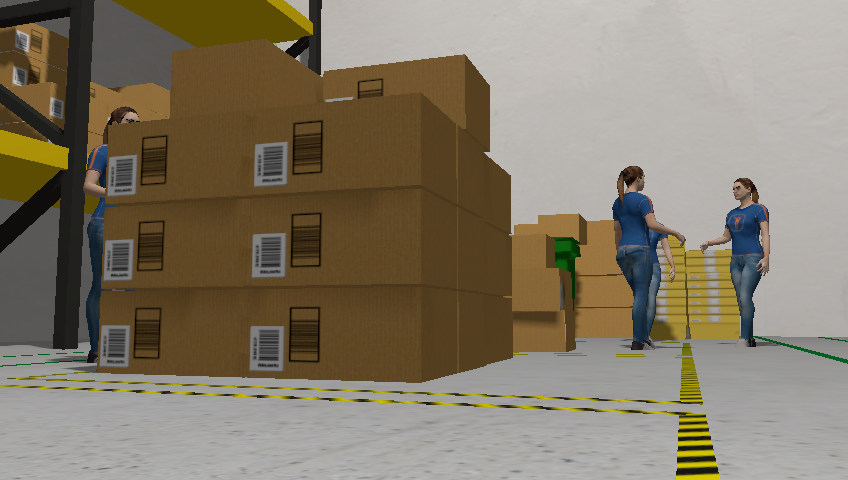
\includegraphics[width=\linewidth]{figures/sim/rgb_img.png}
        \caption{RGB image}
        \label{fig:robot_view_scenario:rgb_image}
    \end{subfigure}
    \begin{subfigure}[h]{0.45\linewidth}
        \centering
        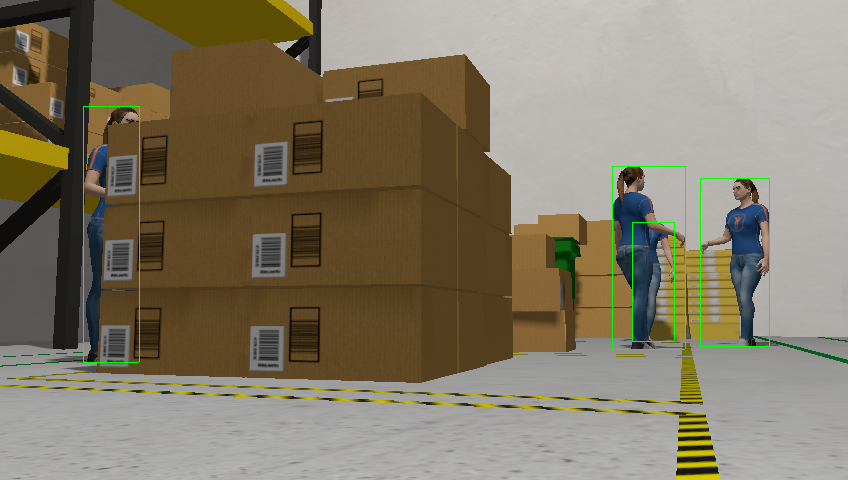
\includegraphics[width=\linewidth]{figures/sim/bbgt.png}
        \caption{Bounding box ground truth}
        \label{fig:robot_view_scenario:bbgt}
    \end{subfigure}
    \caption{Robot view of the simulated scenario}
    \label{fig:robot_view_scenario}
\end{figure}

It is worth pointing out that no dynamic obstacles are implemented in the simulated scenario. However, the \gls{amr} is dynamic and the camera sensors are mounted on top of it. Therefore, in the viewpoint of the \gls{amr}, the obstacles are constantly moving and thus could be treated as dynamic solely for the object detection task. Another reason for this is that the fresh out-of-box bounding box sensor from \gls{gazebo} is inaccurate for dynamic obstacles like humans because dynamic human actors are implemented as the actors in \gls{gazebo} and the animation of the actors is realized by the deformation of the meshes of the actor model. Unfortunately, the bounding box sensor can only provide the bounding boxes of the undeformed actor. Therefore, the bounding boxes available are not accurate to serve as the ground truth for the object detection task. Till the finish of the thesis, the problem is not resolved with the current version of \gls{gazebo} this thesis uses. However, static human obstacles and dynamic \gls{amr} still constitute an adequate simulated scenario for the research questions this thesis is trying to address. 

\subsection{Record and Replay}

% describes how the ROS bag is recorded and how is it replayed during the experiments and explain why this is needed. 
The simulation takes up a great amount of the resources of computers. To reduce the overhead of running the simulation alongside the experiments, this thesis records the simulation to a \gls{ros} bag and replays it during the experiment runs. This reduces the \gls{cpu} and memory usage of the host machine during the experiment and improves the performance of the rest of the offloading pipeline. As mentioned in (TODO: add a reference here), \gls{ros} provides the functionality to record the topics and allows the users to replay them later while preserving the same publishing rate and order of the messages. More importantly, this thesis conduct experiment on a real robotic system with limited resources. Such a system is not capable of running real-time simulations while maintaining the rest of the offloading pipeline. In real-world applications, \glspl{amr} only needs to maintain the driver of the camera and minimal software to be able to get the same image input. In \cref{tab:ros_bag_comparison}, this thesis presents an experiment comparing the \gls{cpu} usage of replaying a \gls{ros} bag and running the library for the Intel RealSense camera. The results show that the two processes have comparable \gls{cpu} usage on a robotic system. Furthermore, \gls{gazebo} slows down the simulation time compared to real-time when the system is strained. Therefore, to ensure a real-time simulation, specifying a replay rate of the \gls{ros} bag can guarantee the simulation time factor is within a reasonable range. 

\begin{table}[htp]
    \centering
    \begin{tabular}{lc}
    \toprule
    Process&                    CPU usage\\
    \midrule
    \gls{ros} bag replay&       14.12\%\\
    RealSense camera library&   11.28\%\\
    \bottomrule
    \end{tabular}
    \caption{Comparison of CPU usage on robotic system}
    \label{tab:ros_bag_comparison}
\end{table}

All topics during the simulation are recorded in the \gls{ros} bag, including the RGB images, the bounding box ground truth, the camera information, etc. The image stream consists of 1748 frames and the \gls{ros} bag is replayed at around 25 frames per second during the experiment. Topics for RGB image stream and the bounding box ground truth are replayed with best effort reliability setting to ensure the RGB images are replayed the same way it is recorded. Since the \gls{ros} topics are recorded at a different time than the experiment, the time stamps of the RGB image messages and the ground truth messages have to be overwritten by the receiving time of the offloading module.

% ---------------------------------------------------------------
\section{Experimental Setup}\label{sec:experiment:experiment_setup}
% ---------------------------------------------------------------

\subsection{Simulation experiment setup}

The host machine is equipped with an Intel(R) Core(TM) i9-7900X \gls{cpu} and a Nvidia GeForce GTX 1060 6GB \gls{gpu}. The \gls{cpu} has a total of 20 cores. In order to simulate the \gls{amr}'s and the edge computer in realistic conditions, this thesis limits the computation resources of the \gls{docker} containers. The robot container is constrained to using only eight cores of the host machine, while the edge container is given ten cores. In addition, the edge computer has the access to the \gls{gpu} of the host machine and calculates the image inference on the \gls{gpu}. Moreover, the robot container is also constrained to using only 4 GB of memory, while the memory of the edge container is not constrained and the host machine has access to 32 GB of memory, including the 4 GB memory assigned to the robot container.

The limitations of CPU and memory usage are realized by tools provided by \gls{docker} itself. According to the \gls{docker} documentation, the runtime memory limitation is realized by Memory Resource Controller provided by the \gls{linux} kernel. Furthermore, the \gls{docker} container can enforce hard memory limitation and soft memory limitation at runtime. The former does not allow the container to use any amount more than specified, while the latter only kicks in when certain conditions are met. In this thesis, we use the hard memory limitation on the robot container to simulate the hardware constraints. For CPU usage, the limitation is realized by the CFS scheduler, which is the \gls{linux} kernel CPU scheduler for normal \gls{linux} processes. This indicates that the limitation on CPU usage is achieved by limiting the accessible CPU cycles of the \gls{docker} container. The GPU of the host machine is exposed to the \gls{docker} containers using the Nvidia Container Toolkits.

In addition to resource limitation simulation, the network is also simulated to achieve realistic conditions for the robot and edge containers. The containers use the default \gls{docker} bridge network. Since the simulated scenario \gls{ros} bag is replayed in the robot container and the output data are also recorded in the robot container, the data flow between the robot container and the edge container only consists of offloaded images and detection processed by the edge container. To allow the data flow of 30 frames per second of images with resolution of 848 x 640 pixels, which is around 40 MB per second, the packet limit of in and out policies of the \gls{netem} is set to 20000. The in and out delays are set to 50 ms for both policies. To investigate the influence of the network bandwidth, the experiments are carried out under two bandwidth conditions: with 160 Mbit/s bandwidth constraint and no bandwidth constraints at all. The former aims to represent a limited network bandwidth that is unable to handle the data flow that is needed for a full offloaded execution, while the latter one represents a unlimited network bandwidth. 

For \gls{qos} settings, the offloading module uses "best effort" reliable policy to prevent the the publisher from being blocked by the bag network connection caused by the bandwidth constraints. As mentioned in (TODO: add a reference here), only \gls{fast_dds} allows a true asynchronous publishing mode. Therefore, Fast-DDS is used for \gls{ros} middle ware and the publishing mode is set to asynchronous for the experiments. The offloading module uses the "keep last" queuing settings and the queue size is set to 5. Furthermore, the \gls{ros} bag replay of the simulated scenario and the state monitors also use "best effort" reliable policy settings to simulate a camera sensor. 

\subsection{Robot experiment setup}

Unlike the simulation experiments, described in (TODO: add a reference here), the real-robot experiment uses two separate computers for the \gls{amr}'s onboard system and the edge computer. For the robot, the onboard system uses a \gls{nuc} equipped with an Intel(R) Core(TM) i3-8109U \gls{cpu}, which is commonly used for \glspl{amr}.  For the edge, a \gls{linux} desktop computer equipped with an Intel(R) Core(TM) i3-8109U \gls{cpu} and a Nvidia GeForce GTX 1060 6GB \gls{gpu} is used. On both computers, the offloading module and the perception modules have full access to the available resources. The distribution of the modules between the two computers is illustrated in (TODO: add a reference here). The \gls{ros} bag replay of the simulated scenario is carried out on the robot. The output data of the metrics are also recorded on the robot. The edge computer is solely responsible for the inference of the offloaded images and monitoring the edge system states and sending them to the robot. The image inference is computed by the \gls{gpu} on the edge computer with help of \gls{pytorch} library, while the image inference on the robot is computed by its onboard \gls{cpu}. As mentioned in (TODO: add a reference here), the system states of the robot and the edge are measured with the "system status" package.

% TODO: add a photo of nuc is this figure
% \begin{figure}
%     \centering
%     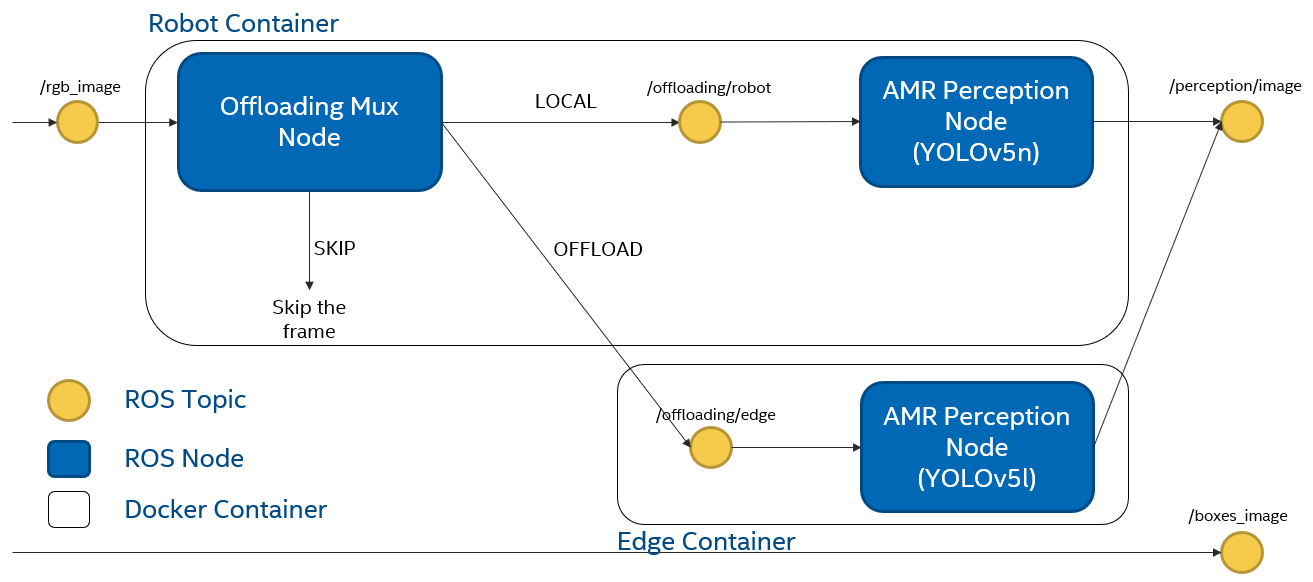
\includegraphics[width=\linewidth]{figures/setup/general_setup.png}  % TODO: change here
%     \caption{Setup for real-robot experiment (TODO: adapt this fig)}  % TODO: change here
%     \label{fig:real_robot_experiment_setup}  % TODO: change here
% \end{figure}

Two network interfaces are used to conduct the real-robot experiments. First, the experiment uses an Ethernet connection between the two computers. Similar to the simulation experiments, two network conditions are tested under the Ethernet connection. First, an Ethernet network interface without bandwidth constraints is used to simulate a perfect network connection between the robot and the edge. Then, the Ethernet network interface is constrained to 160 Mbits/s bandwidth to simulate a bag network connection. Finally, a \gls{wifi} network interface is used the carry out the experiment. The \gls{wifi} network has unstable network bandwidth from time to time and therefore affects the experiment results drastically. This is to investigate different offloading strategies under dynamic network condition changes. When conducting the experiment with one network interface, the other one is shutdown to avoid the offloading pipeline uses both network interfaces simultaneously. 

Similar to simulation experiment, \gls{fast_dds} is used as middle ware for \gls{ros}.The \gls{qos} reliability policy for offloading is set to "best effort" and the publishing mode of \gls{fast_dds} is set to asynchronous to avoid the publisher blocked by the network. Moreover, the queuing settings use "keep last" policy and the queue size is set to five messages. Under various \gls{qos} settings, this setup achieves the best performance of the object detection task. However, other \gls{qos} settings are also investigated during the experiments. In (TODO: add a reference here), the results of the experiment with "reliable" reliability policy are presented. 


\section{Evaluation Framework}

\subsection{Metrics}
% This section lists all the evaluation metrics used and how they are recorded and what tools are used in order to record them. 

% TODO: rewrite this section with more specifications on how the metrics are measured. Maybe list all metrics in itemized order. 

The evaluation metrics used by this thesis fall into two categories. The second category focuses mainly on the resources of the \gls{amr}. This includes the CPU percentage, the power consumption, and the network throughput. These metrics represent the onboard resources for computation, energy, and network used by the \gls{amr}. For these metrics, this thesis also includes the results when the offloading pipeline is idling as a baseline to eliminate the influence of processes other than the perception modules on the metrics. More specifically, in the baseline, the offloading module and the perception modules are still launched and the ROS bag is also being replayed. However, the offloading module is not sending any messages to the onboard perception module or the edge perception module, i.e., there are no object detection tasks being performed at all. 

The second category describes the performance of the object detection task, including the execution latency, the overall processed frame rate, and the \gls{map}. The two components of the execution latency, i.e., the network delay and the inference time, are evaluated separately for offloading and local computation. In addition, to evaluate how the offloading pipeline is performing over the entire simulation, the overall processed frame rate, i.e., what percentage of all the frames are processed by perception modules. The \gls{map} only consider the person class in the obstacles. The detection from the perception modules is compared with the bounding box ground truth from the simulation. The evaluation algorithm is provided by the package "torchauto" as a part of the code base from \gls{amsrl}. 

For the comparison between the detection and the ground truth, the time stamps of the messages are crucial to the final result. This raises the question: what should be considered as simultaneity for the detection and the ground truth in task offloading? This thesis presents two evaluation methods of the \gls{map} metric in order to gain some insights into this question. 

\subsection{Evaluation methods}

\begin{figure}[htp]
    \centering
    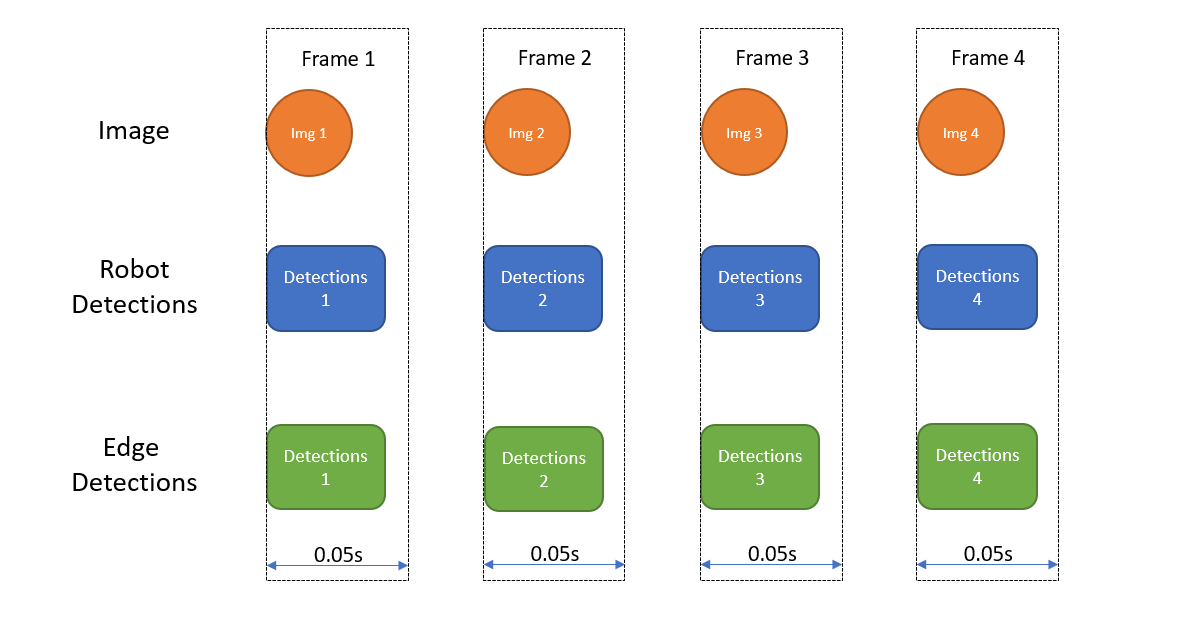
\includegraphics[width=\linewidth]{figures/setup/sync_eval.png}
    \caption{Synchronous evaluation}
    \label{fig:sync_eval}
\end{figure}

In the synchronous evaluation, the detection is evaluated by being compared with the ground truth of the same time stamp. As illustrated in \cref{fig:sync_eval}, the image is either processed by the robot perception module or the edge perception module. The processed result and the ground truth are recorded by the ROS bag. After the experiment runs, the recorded result and the ground truth with the nearest time stamps are grouped as one data frame by the message filter. The message filter groups the messages from different ROS topics. The proximate messages within a time threshold can be considered as the same data frame. The threshold is currently set to 0.05 seconds. The \gls{map} is calculated within the same data frame. For the entire experiment run, the mean and the standard deviation are calculated for all the data frames. This means the data frame is discarded if no detection or ground truth is present for the specific time stamp, i.e., the \gls{map} will not be affected if the robot onboard system or the edge computer is not capable of processing the image. The capability of processing the image is however reflected in the metric of the overall processed frame percentage. 

The synchronous evaluation method does not take the execution latency into consideration, because the detection is compared against the ground truth with the same time stamp as the original image. Therefore, the final result interpolates the \glspl{map} of the edge computer and the robot onboard system. However, this also does not represent the offloading scenario accurately. In real-world applications, the \glspl{amr} move continuously. The current situation of the \gls{amr} could be very different than the moment the image is taken by the camera if the processing takes too long and the detection is outdated. Therefore, the execution latency plays an important role in the accuracy of how well the \glspl{amr} perceives the environment. 

With the aforementioned considerations, this thesis investigates an asynchronous evaluation method that takes the execution latency into consideration, which is the evaluation method for \gls{map} metric that the thesis adopts. As illustrated in \cref{fig:async_eval}, the detection is compared against the images with the time stamps when the \glspl{amr} actually receive the processed result. This is achieved by changing the time stamps of the detection messages to the receiving time of the \glspl{amr}. Depending on how much the images have changed, the quality of the detection deteriorates with the execution latency, which is usually the case in real-world applications.

\begin{figure}[htp]
    \centering
    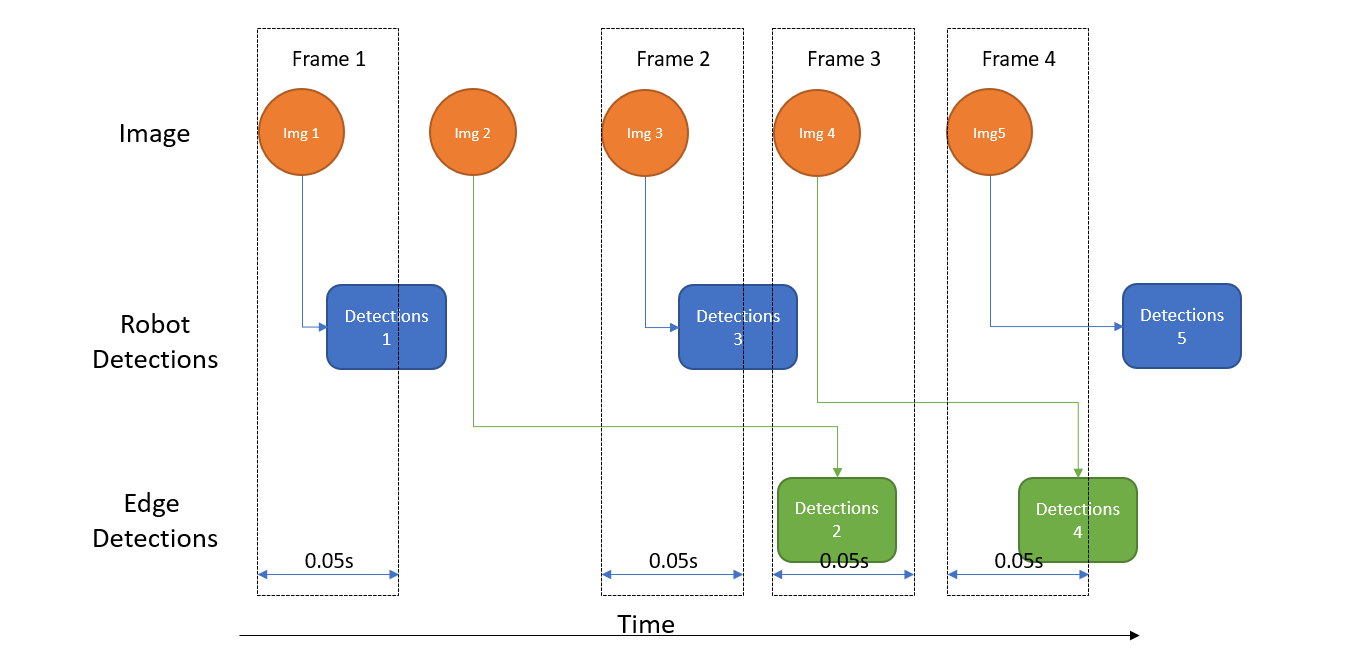
\includegraphics[width=\linewidth]{figures/setup/async_eval.png}
    \caption{Asynchronous evaluation}
    \label{fig:async_eval}
\end{figure}

% -----------------------------------------------
\section{Analysis}\label{sec:experiment:analysis}
% -----------------------------------------------

\subsection{Simulation experiment}

\subsection{Robot experiment}

When the network condition is not constrained, the "edge only" strategy shows the best results in the object detection task, as shown in \cref{fig:real_robot_experiment:eth_map}. This is mainly caused by two reasons. On one hand, the edge computer is using the more complex network, i.e., \gls{yolov5}l, which provides a more precision detection. On the other hand, even though the \gls{rtt} of the edge perception is still higher than the robot perception, the difference is still relatively low, as shown in \cref{fig:real_robot_experiment:eth_rtt}. Therefore, the inaccuracy caused by the execution delay is negligible. Moreover, the "edge only" strategy also processed the most frames in the experiments. This also makes the "edge only" strategy the safest among different strategies. With more detection frames, the \gls{amr} is able to adapt its behavior to the detection more quickly. The "edge only" strategy also uses the least \gls{cpu} and energy of the onboard system, since the images are exclusively calculated on the edge computer. This is beneficial to \gls{amr}'s onboard system and battery life. This also allows the \glspl{amr} to free up more resources for other tasks, e.g., \gls{slam}, navigation, and path planning. However, the "edge only" strategy also uses the most network bandwidth. For image feed with 30 \gls{fps} at a resolution of 848x640 pixels, around (TODO: add a number here) MB/s bandwidth is used for offloading. Such bandwidth will be a huge amount for wireless connection. For comparison, IEEE IEEE 802.11ac (\gls{wifi} 5G) can support only up to (TODO: add a number here) bandwidth. If the number of the \glspl{amr} scales, the network cannot provide such bandwidth. Therefore, "edge only" strategy is not suitable for industrial usage. 

% Figure for eth mAP
\begin{figure}
    \centering
    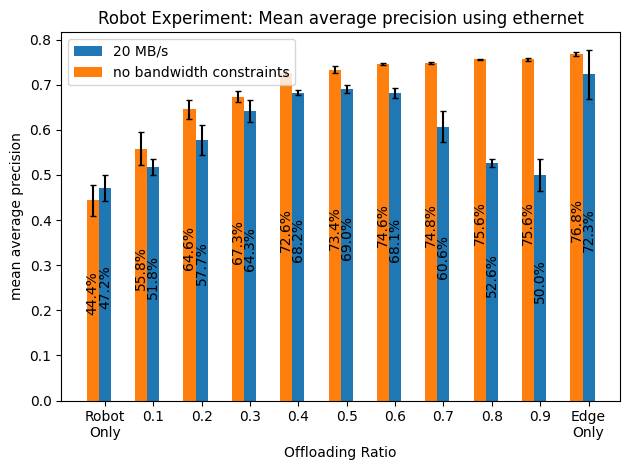
\includegraphics[width=\linewidth]{figures/experiment/real_robot/eth/map.png}
    \caption{Real-robot experiment: \gls{map} with Ethernet}
    \label{fig:real_robot_experiment:eth_map}
\end{figure}

On the other hand, the "robot only" strategy delivers the worst results in the object detection task. This is mainly because the onboard resources are not enough for the \gls{amr} to process all the images. The robot perception module is strained when more images are calculated locally on the \gls{amr}'s onboard system. As shown in \cref{fig:real_robot_experiment:eth_rtt}, the robot perception has the highest \gls{rtt} with "robot only" strategy. The \gls{rtt} of robot perception is broken down to different components in \cref{fig:real_robot_experiment:eth_execution_time_320}. The inference time of the robot perception stays the same. However, the network delay is increased. This indicates that the robot perception module has too many images waiting for processing and the images start to queue, causing the network latency of robot perception to increase. As shown in \cref{fig:real_robot_experiment:eth_execution_time_320}, the network latency of robot perception stabilizes around 0.6 offloading ratio. This infers that the \gls{amr}'s onboard system, i.e., the \gls{nuc}, is only able to process less than 40 percent of the offloaded images, i.e., around 12 \gls{fps}. This corresponds to the 99.9 ms \gls{rtt} of the robot perception at offloading ratio 0.6, as shown in \cref{fig:real_robot_experiment:eth_rtt}. Naturally, the "robot only" strategy also uses the most \gls{cpu} and energy, since it computes the all images onboard, as shown in \cref{fig:real_robot_experiment:eth_cpu_percentage} and \cref{fig:real_robot_experiment:eth_cpu_energy_consumption}. Moreover, the "robot only" strategy uses the least network bandwidth. It still uses 0.4 MB/s network bandwidth because the states monitors need to send system state data from the edge computer to the \gls{amr}'s onboard system.

As illustrated in \cref{fig:real_robot_experiment:eth_map}, the \gls{map} of the object detection task saturates between offloading ratios 0.5 and 0.8. This indicates that both the robot perception and the edge perception are working under their optimal workload. The task performance reaches a stationary point. After the stationary point, the edge perception becomes more prominent for the performance. Therefore, the performance continues to improve due to the more accurate object detection of the more complex model on the edge. 

The decision-making strategy also delivers decent results for the object detection task under good network condition. As shown in \cref{fig:real_robot_experiment:eth_processed_frame_percentage_320}, the decision-making strategy offloads most images to the edge computer and only computes (TODO: add a number here) on the \gls{amr}'s onboard system. This decision can be justified by the low \gls{rtt} of the edge computer. (TODO: add analysis after getting the results). It it worth noticing that decision-making strategy calculates a small portion of the images locally on the onboard system, since the \gls{rtt} of edge perception can increase temporarily due to dynamic changes in the network. However, because the network condition is good, most of the images are offloaded to the edge computer. 

% Figure for eth RTT
\begin{figure}
    \centering
    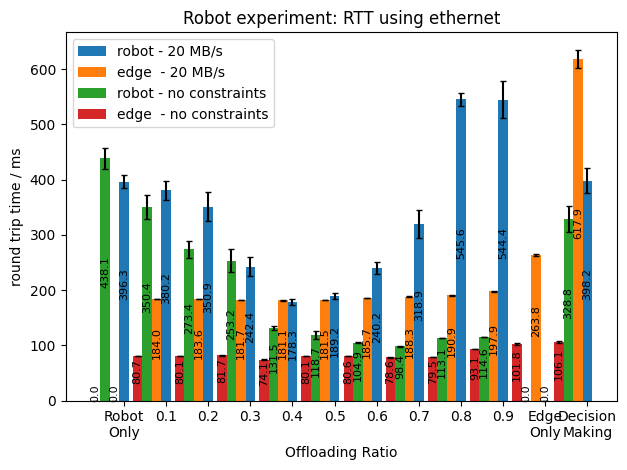
\includegraphics[width=\linewidth]{figures/experiment/real_robot/eth/RTT.png}
    \caption{Real-robot experiment: \gls{rtt} with Ethernet}
    \label{fig:real_robot_experiment:eth_rtt}
\end{figure}

When the network condition is constrained, the "edge only" strategy does not provide the best \gls{map} among all strategies. Since the network is not capable of transmitting the amount of data the strategy needs, the messages starts to queue and the "best effort" reliable policy allows the middleware to drop many messages. This can be visualized in \cref{fig:real_robot_experiment:eth_execution_time_160} and \cref{fig:real_robot_experiment:eth_processed_frame_percentage_160}. The processed frame percentage starts to drop drastically after the offloading ratio exceeds 0.5 and the network latency of the edge perception increases. This also corresponds to the network bandwidth in \cref{fig:real_robot_experiment:eth_bandwidth}. The network bandwidth is at its capacity after the offloading ratio exceed 0.5. Furthermore, with the offloaded images hogging the network bandwidth, it is unlikely for the \glspl{amr} to transmit other data over the network, which can be essential for the safety of the \glspl{amr}. This makes "edge only" strategy the worst strategy under constrained network condition. 

On the other hand, the "robot only" strategy delivers similar results under the two network conditions. Since the "robot only" strategy compute the object detection locally on the onboard system, the performance should be independent from the network conditions. However, it is worth noticing that the there is a slight performance drop for all strategies up to offloading ratio 0.5 due to a slight increase of the network latency on the robot perception. It is suspected that the \gls{netem} layer affects the \gls{ros} middleware and thus causes a increased latency in transmitting the data between the offloading module and the robot perception module. 

The best performance of \gls{map} occurs around offloading ratio of 0.5. At this offloading ratio, the network bandwidth has not exceeded its limits and the robot perception is able to process the given workload. Therefore, the \glspl{rtt} of both perception modules are low and the \gls{amr} is able to get the detection in time. Moreover, offloading at this ratio also allows the \gls{amr} to use less onboard resource, as shown in \cref{fig:real_robot_experiment:eth_cpu_percentage} and \cref{fig:real_robot_experiment:eth_cpu_energy_consumption}. Therefore, under constrained network condition, offloading a portion of the images is the best strategy. However, the offloading ratio is dependent on the available network bandwidth and the computation capabilities of the \gls{amr}'s onboard system.

% Under constrained network condition, the decision-making strategy also managed to deliver decent results. The increased \gls{rtt} time forces the \gls{amr} to compute most of the images locally. However, the decision-making strategy still offloads a portion of the images to the onboard system, because the onboard system is not able to process all images and \gls{rtt} of the robot perception will increase drastically if the images start to queue. These results show that the decision-making strategy is able adapt to the dynamic changes of the network by simply using the \gls{rtt} as a criterion. Furthermore, the \gls{amr} uses more \gls{cpu} and energy with the decision-making strategy under constrained network condition compared to unconstrained network condition, since the \glspl{amr} have to do more computation on the board system and thus consume more onboard resources, as shown in \cref{fig:real_robot_experiment:eth_cpu_energy_consumption} and \cref{fig:real_robot_experiment:eth_cpu_percentage}.

% Figure for eth execution time 160M
\begin{figure}
    \centering
    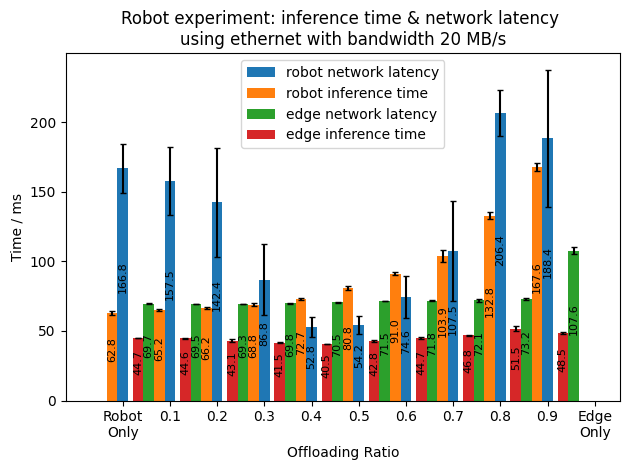
\includegraphics[width=\linewidth]{figures/experiment/real_robot/eth/execution_time_160.png}
    \caption{Real-robot experiment: execution times with Ethernet with 160 Mbits/s bandwidth}
    \label{fig:real_robot_experiment:eth_execution_time_160}
\end{figure}

% Figure for eth execution time 320M
\begin{figure}
    \centering
    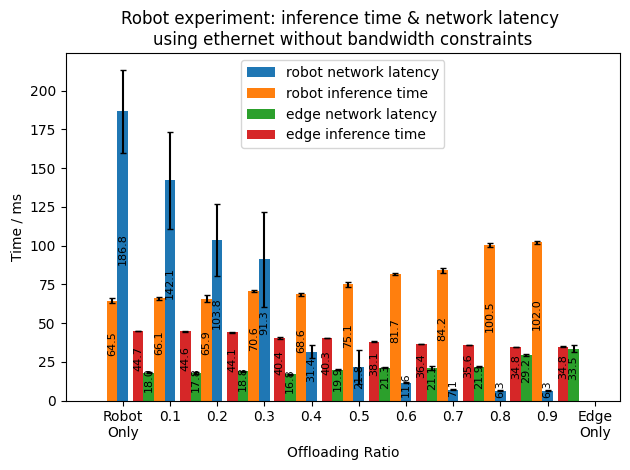
\includegraphics[width=\linewidth]{figures/experiment/real_robot/eth/execution_time_320.png}
    \caption{Real-robot experiment: execution times with Ethernet with 320 Mbits/s bandwidth}
    \label{fig:real_robot_experiment:eth_execution_time_320}
\end{figure}

% Figure for eth overall processed image percentage
\begin{figure}
    \centering
    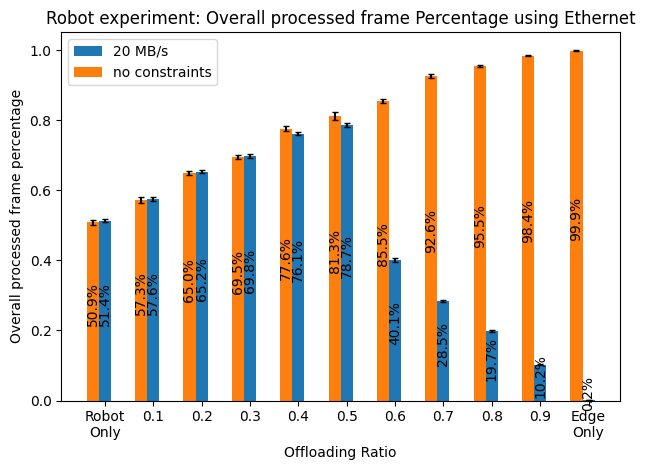
\includegraphics[width=\linewidth]{figures/experiment/real_robot/eth/overall_processed_frame_percentage.png}
    \caption{Real-robot experiment: overall processed frame percentage with Ethernet}
    \label{fig:real_robot_experiment:eth_overall_processed_frame_percentage}
\end{figure}

% Figure for eth processed image percentage 160M
\begin{figure}
    \centering
    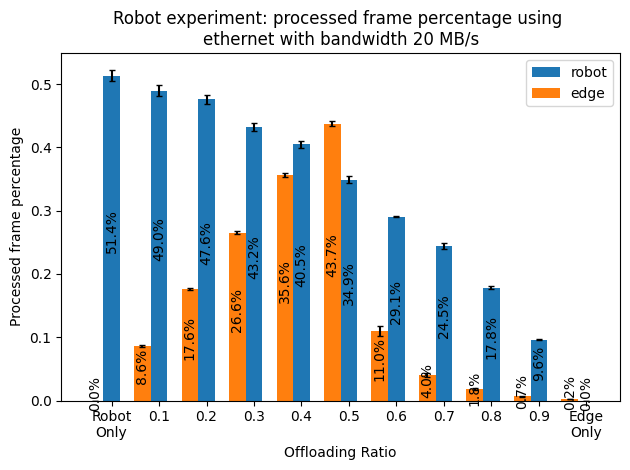
\includegraphics[width=\linewidth]{figures/experiment/real_robot/eth/frame_percentage_160.png}
    \caption{Real-robot experiment: processed percentage with Ethernet with 160 Mbits/s bandwidth}
    \label{fig:real_robot_experiment:eth_processed_frame_percentage_160}
\end{figure}

% Figure for eth processed image percentage 320M
\begin{figure}
    \centering
    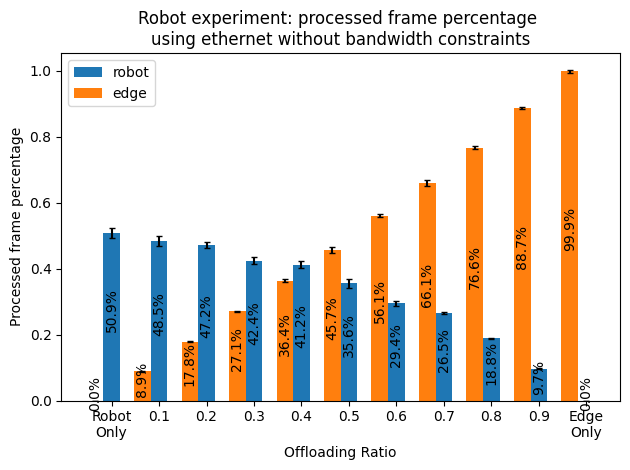
\includegraphics[width=\linewidth]{figures/experiment/real_robot/eth/frame_percentage_320.png}
    \caption{Real-robot experiment: processed percentage with Ethernet with 320 Mbits/s bandwidth}
    \label{fig:real_robot_experiment:eth_processed_frame_percentage_320}
\end{figure}

% Figure for CPU percentage
\begin{figure}
    \centering
    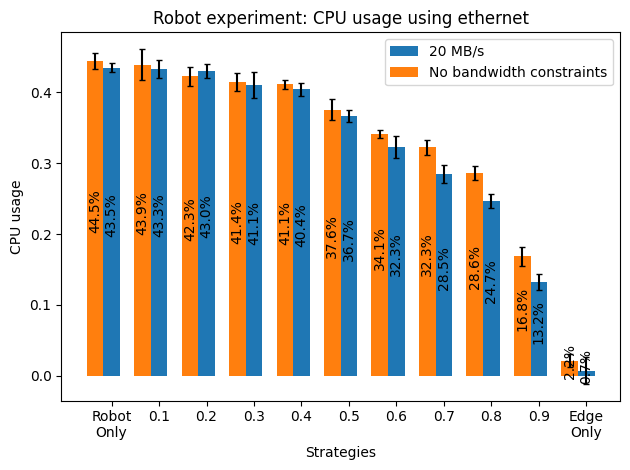
\includegraphics[width=\linewidth]{figures/experiment/real_robot/eth/cpu_percentage.png}
    \caption{Real-robot experiment: CPU usage using Ethernet}
    \label{fig:real_robot_experiment:eth_cpu_percentage}
\end{figure}

% Figure for CPU energy consumption
\begin{figure}
    \centering
    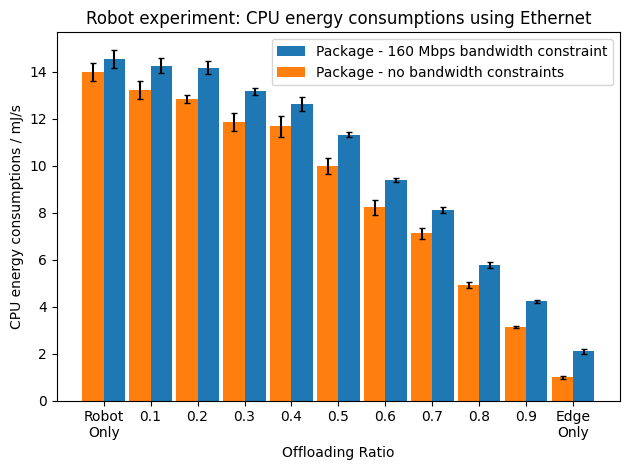
\includegraphics[width=\linewidth]{figures/experiment/real_robot/eth/cpu_energy_consumption.png}
    \caption{Real-robot experiment: CPU energy consumption using Ethernet}
    \label{fig:real_robot_experiment:eth_cpu_energy_consumption}
\end{figure}

% Figure for network bandwidth
\begin{figure}
    \centering
    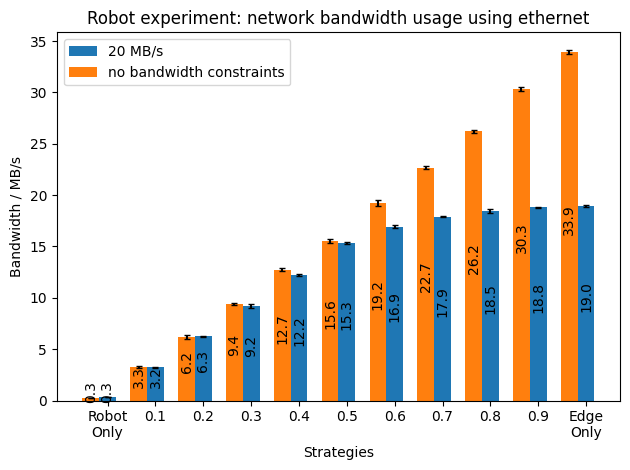
\includegraphics[width=\linewidth]{figures/experiment/real_robot/eth/bandwidth.png}
    \caption{Real-robot experiment: network bandwidth usage using Ethernet}
    \label{fig:real_robot_experiment:eth_bandwidth}
\end{figure}

\chapter{Conclusion and Future Work}\label{ch:conclusion}

% ---------------------------------------------------------------
\section{Summary and Discussion}\label{sec:discussion}
% ---------------------------------------------------------------

In order to investigate the influence of different offloading strategies on the important metrics of the \glspl{amr}, this thesis designs and implements an offloading framework for perception offloading using \gls{ros}. The robotic perception task is chosen to use \gls{yolo}v5 algorithms with an image stream with a frame rate of around 25 FPS and a resolution of 848 by 480 pixels. The bandwidth usage of an entire computation offloading can amount to 244 Mbps. To balance the computation resources of the two systems and the execution latency of the object detection task. Two models with different sizes are chosen respectively for the \gls{amr}'s onboard system and the edge computer. 

Afterward, this thesis implements the baseline offloading strategies and conducted experiments in simulation. In order to carry out the experiment, a simulated scenario of a factory warehouse is implemented for \glspl{amr} in \gls{gazebo}. Furthermore, different experimental setups are created for experiments in simulation and with actual robotic systems. In addition, this thesis designs and implements an asynchronous evaluation method by considering the actual robotic application of perception offloading. After identifying the \gls{rtt} as an important factor for the performance of the object detection task as well as the \gls{amr}'s onboard system, this thesis implements a dynamic offloading strategy by using \gls{rtt} as an offloading decision-making criterion with the goal of improving the performance of the object detection task and reducing the execution latency as well as the usage of the \gls{amr}'s onboard resources. Finally, this thesis conducts an experiment with an actual robotic system and an edge computer to evaluate the dynamic offloading strategy against the baseline strategies. The experiment is conducted with Ethernet and \gls{wifi} connection. 

The experiment results show that both "edge only" and "robot on" strategies are not ideal for computing time-sensitive tasks like object detection. Moreover, the results show that the offloading ratio is dependent on the available onboard resources and the network condition for a partially offloading strategy. From the robot experiments, the dynamic offloading strategy shows the ability to adapt to dynamic network changes and improves the metrics compared to baseline strategies. More specifically, the dynamic offloading strategy improves the average precision of the object detection on human class compared to "robot only" and "edge only" strategies, while drastically reducing the \gls{cpu} usage and \gls{cpu} power consumption compared to "robot only" strategy. 

% This thesis investigates the influence of different offloading strategies on important metrics. This thesis is built on the underlying assumptions that the \gls{amr} has limited computation and energy resources on its onboard system and the edge computer has abundant resources. Therefore, offloading some computation tasks to the edge computer can alleviate the situation. As an essential and computationally expensive task, object detection is used as the offloaded task. The state-of-art object detection pre-trained models are used to carry out the experiments. A complete offloading and evaluation pipeline is implemented to investigate the research questions. Different offloading strategies are implemented. Various metrics of the object detection task and the \gls{amr}'s onboard system are identified and defined. Furthermore, an appropriate evaluation method is chosen for the metrics. 

% The experiments are first carried out in simulation to ensure the performance and robustness of the implementation. After simulation experiments, the \gls{rtt} is identified as an important factor for the performance of the object detection task. Therefore, it is used as a criterion for offloading decisions in the decision-making strategy. Finally, the experiments are conducted using a robotic system and an edge computer. The experiments are also carried out with both Ethernet and \gls{wifi} connections. The results from the experiments show that the performance of the object detection task is also highly dependent on the available network bandwidth between the \gls{amr} and the edge computer. When the network bandwidth is enough for the offloaded task, it makes more sense for the \glspl{amr} to offload the task to the edge. This not only improves the task performance, e.g., higher processed frame rate, better \gls{ap}, etc but also reduce the resource usage on the \gls{amr}, e.g., \gls{cpu} usage and power consumption. This is beneficial for the \glspl{amr} in many ways. First, better performance of the object detection task will improve the \gls{amr}'s perception of the environment. More accurate perception makes the \glspl{amr} less unlikely to collide with obstacles. A higher frame rate allows the \glspl{amr} to adapt earlier changes to its behavior. These improvements will allow the \glspl{amr} to operate more safely. Moreover, by offloading the computationally expensive tasks to the edge computer, the \glspl{amr} have more available onboard resources, e.g., CPU cycles, and battery life. This ensures an efficient operation and increases the availability of the \glspl{amr}. Furthermore, with more onboard resources freed up, the \glspl{amr} can use them for other safety-critical tasks onboard, e.g., \gls{slam}, navigation, etc. This also increases the safety of the \glspl{amr} indirectly.

% However, if the network bandwidth is constrained, offloading all of the tasks may cause network congestion. The network delay of the edge perception will increase drastically and the performance of the object detection task of the images processed by edge computer will deteriorate. Under heavy load, the edge computer can only return a small number of processed detection with high network latency. In this case, the detection processed by the edge is essentially unusable. Moreover, if the network is bogarted by the offloaded task, other data cannot be transmitted over the network, which can be essential for other tasks of the \glspl{amr}, e.g., navigation, emergency control, etc. Therefore, the safety of the \glspl{amr} can be affected. However, offloading a portion of the object detection task within the limits of the network bandwidth will increase the performance of the object detection task and reduce the usage of the onboard resources. How much of the task should be offloaded to the edge computer is also dependent on the available network bandwidth and the available resources onboard. This can vary among different machines. In general, the offloading strategy can be considered as a compromise between the available onboard resources and the available network bandwidth. 

% The thesis also implements a dynamic offloading strategy that uses the states of the onboard system and the network to decide whether to offload. The \gls{rtt} is used as a criterion for offloading decisions. As mentioned in (TODO: add reference here), \gls{rtt} consists of the network latency and the inference time. This value represents both the computation capacities of the system and the network condition. If the system does not have enough computation resources, it will take more time to do the inference and thus cause the \gls{rtt} to increase. If the network is congested, the network latency of the task will increase because the task will start to queue. Therefore, the dynamic offloading strategy uses \gls{rtt} as a criterion for offloading decision. The results from the experiments show that this strategy can already handle different network bandwidth. Hence, this answers another research question: Is more complex offloading strategy justified? For time-sensitive tasks, such as object detection, \gls{slam}, more complex offloading strategy, such as \gls{drl}, will increases the execution latency. For comparison, the simplest object detection model \gls{yolo}v5n takes 50.88 ms to do inference on one image, as presented in \cref{tab:inference_time} on the \gls{nuc}. It's reasonable to assume that a \gls{drl} model will use comparable time as well. However, the \gls{rtt} of the edge perception under unconstrained network is less than 100 ms. If a \gls{drl} agent is adopted as the offloading module, the \gls{rtt} can easily increase by 50 percent. In such case, the performance of the object detection task will deteriorate drastically. 

% ------------------------------------------
\section{Limitations}\label{sec:limitations}
% ------------------------------------------

% Since this thesis uses pre-trained object detection models from \gls{yolo}v5, only the human obstacles are used to evaluate the \gls{ap}. Other obstacles, such as shelves, boxes, and pallets, are not considered in the evaluation because they are not in the \gls{coco} dataset and cannot be detected by the pre-trained models accurately. They are only used to increase the complexity of the object detection task. For example, some of the human obstacles are partially occluded by other obstacles. Furthermore, to retrieve ground truth data from \gls{gazebo} simulation, the human obstacles are static in the simulated scenario. Due to technical issues, the bounding box ground truth of dynamic objects in \gls{gazebo} cannot be a

The pre-trained \gls{yolo}v5 object detection models impose some limitations on the evaluation of the experiment results. Since the pre-trained models are trained with \gls{coco} dataset, only the person class can be accurately detected. Other obstacles, such as shelves, boxes, and pallets, are not considered in the evaluation of the average precision of the object detection task. However, they still contribute to the complexity of the simulation scenario by providing false positive detections and occlusions, as discussed in \cref{sec:simulated_scenario}. 

Another limitation results from the \gls{gazebo} simulation. Due to technical issues, the bounding box camera sensor in \gls{gazebo} cannot generate accurate bounding box ground truth for moving actors in \gls{gazebo}. However, to the author's knowledge, dynamic human obstacles can only be implemented as actors in \gls{gazebo}. Therefore, the human obstacles are static in the simulated scenario. Luckily, the \gls{amr} is implemented dynamically in the simulated scenario. In the view of the camera, the human obstacles are still static. However, this still imposes some limitations on the simulated scenario since the animation of the human obstacles is disabled. 

% -------------------------------------------
\section{Future Work}\label{sec:future_works}
% -------------------------------------------

Foremost, the offloading pipeline is implemented in an open-loop manner, i.e., the processed results are not used for downstream applications. In future works, the object detection results can be used for obstacle avoidance and local path planning to increase the \gls{amr}'s safety. This will allow the offloading strategy to modify the behavior of the \gls{amr} and create more meaningful metrics for offloading strategies, e.g., safety metrics. The experiment can measure the times when the \glspl{amr} collides with an obstacle.

Additionally, this thesis only considers the scenario where one \gls{amr} offloads to one edge computer to reduce the complexity in evaluation. For future works, the number of the \glspl{amr} can also be increased while there is still only one edge computer. Within the work of this thesis, the bandwidth constraints are achieved by limiting the available bandwidth between the \gls{amr} and the edge computer. However, in real-world applications, the \glspl{amr} will also compete over the available bandwidth of the edge computer. In that case, the dynamic offloading strategy will also have to consider such competition between \glspl{amr}. For example, the game-theory approaches, described in \cref{sec:game_theory_approaches}, can be considered for reconciling the resource competition among multiple \glspl{amr}. Furthermore, other metrics can be considered for multi-robot offloading, such as the joint efficiency that measures the overall energy consumption and the network bandwidth usage.

% First, this thesis only considers the scenario where one \gls{amr} offloads to one edge computer to reduce the complexity in evaluation. In real-world application, the \glspl{amr} and edge computers are usually deployed in swarms. Therefore, the \gls{amr} also has to decide to which edge computer it offloads. The one-robot-one-edge-computer also simplify



%
% Appendix
% --------
\appendix%
\chapter{Results for Robot Experiment with Reliable QoS Reliability Policy}\label{ch:appendix_a}

The experiment with the actual robotic system is also carried out in reliable \gls{qos} reliability policy. The \gls{ros} middleware still uses \gls{fast_dds}. The Ethernet connection is used and the bandwidth is constrained to 160 Mbps by \gls{netem}. 

The results are shown in \cref{tab:dynamic_eth_reliable}. In general, the performance of the object detection task is lower compared to using the best effort \gls{qos} reliability policy. The best offloading ratio occurs at 0.2. Since the reliable policy requires a confirmation of the receipt of the message, both robot and edge \glspl{rtt} take longer. The "edge only" strategy cannot process any frames. Therefore, it does not have any measurement in terms of object detection performance. The dynamic offloading strategy still manages to adapt to these network changes and outperforms the "robot only" strategy by $1.5\%$ in \gls{ap}. 

 % Table for dynamic offloading strategy with 160 Mbps bandwidth constraint
\begin{table}[htb]%
    \centering%
    \footnotesize
    \begin{tabular}{l|ccc|c}
        \toprule
        Strategies &                        Robot only &            Edge only &             Best among ratios &                dynamic offloading \\
        \midrule
        \gls{ap} &                          $18.08\%\pm0.99\%$ &    $0$ &     $\mathbf{31.01\%\pm1.24\%}$ &        $19.47\%\pm1.54\%$\\
        Robot perception \gls{rtt} / ms &        $1634.72\pm 64.30$ &     / &                     $1781.34\pm142.89$ &          $\mathbf{1594.10\pm109.72}$\\
        Edge perception \gls{rtt} / ms &          / &                    / &         $\mathbf{322.47\pm0.21}$ &            $2517.29\pm257.00$\\
        Processed frames percentage &       $59.87\%\pm2.45\%$ &    $0$ &          $\mathbf{68.88\%\pm0.27\%}$ &        $61.92\%\pm4.07\%$\\
        \midrule
        CPU usage &                         $48.69\% \pm 0.85\%$ &  $\mathbf{6.35\% \pm 0.80\%}$ &    $49.24\% \pm 0.65\%$ &     $48.00\% \pm 0.81\%$ \\
        Power consumption / mJ/s &      $17.17 \pm 0.73$ &      $\mathbf{2.14 \pm 0.09 }$ &       $16.21 \pm 0.05$ &         $16.94 \pm 0.89$\\
        Bandwidth usage / Mbps &            $\mathbf{3.22 \pm 0.14}$ &       $151.73 \pm 0.92$ &      $59.50 \pm 0.77$ &         $12.79 \pm 0.97$ \\
        
        \bottomrule
    \end{tabular}
    \caption{Metrics of dynamic offloading strategy compared with baseline strategies using Ethernet with 160 Mbps bandwidth constraint and reliable \acrshort{qos} reliability policy}
    \label{tab:dynamic_eth_reliable}%
\end{table}

%

%
% References
% ----------
{%
    \sloppy% "Word"-like typesetting in order to improve breaking lines with long URLs/DOIs
    \printbibliography[heading=bibintoc]%
}%
%
%
\end{document}%
%
%
